\documentclass[../main.tex]{subfiles}

\begin{document}

\section{Electrolytes}
\label{sec:electrolytes}
\subsection{Introduction (Arihant)}
\label{sec:electrolytes_introduction}
Electrolytes are a medium for the transport of charged ionic species, i.e. Li$^+$, between the electrodes.\cite{Schmickler2010,Bard2010} While the electrons flow through the outer circuit, an equal ionic current flows through the electrolyte to balance the charge. Electrolytes can be categorised into two groups: liquid and solid, both of which have their benefits and drawbacks. Liquid electrolytes are currently used in commercial lithium ion batteries and offer high conductivities, but have safety concerns.\cite{kralisch2005energetic, smiglak2006combustible,ding2013effects} Solid electrolytes are a safer alternative that are approaching commercialisation and can potentially reach higher energy densities, however, they are yet to match liquids in battery performance. There are several key aspects to the design of either liquid or solid electrolytes in Li-ion batteries: electrochemical stability window,\cite{Goodenough2010, kazemiabnavi2016electrochemical} ionic conductivity,\cite{park2010review,Kamaya2011} electric double layers,\cite{Schmickler2010,Swift2021} solid-electrolyte interphase, \cite{Xu2011,Yu2017} and safety which are discussed in the following sections.\cite{Xu2004,Xu2014}

\textbf{Electrochemical stability window} An electrolyte can be safely used within an electrochemical stability window, which is the voltage range beyond which it can be oxidized or reduced.\cite{Goodenough2010} The electrochemical stability window is schematically depicted in Figure~\ref{fig:electrolyte}, which shows the electronic energy levels in the electrodes and electrolyte of a battery cell. If the anode electrochemical potential, $\mu_{A}$, is above the lowest unoccupied molecular orbital of the electrolyte, the electrolyte will be reduced. Conversely, if the cathode electrochemical potential, $\mu_{C}$, is below the highest occupied molecular orbital of the electrolyte, the electrolyte will be oxidized. Therefore, the electrochemical potentials, $\mu_{A}$ and $\mu_{C}$, should lie within the energy gap, $E_g$, between the LUMO and the HOMO of the electrolyte, which constrains the open-circuit voltage $V_{\rm oc}$ of a battery cell:\cite{Goodenough2010}

\begin{equation}
    eV_{\rm oc}=\mu_{A}-\mu_{C}\leq E_{g},
\end{equation}

where $e$ is the elementary charge or the magnitude of the charge on an electron. 

\begin{figure}
    \centering
    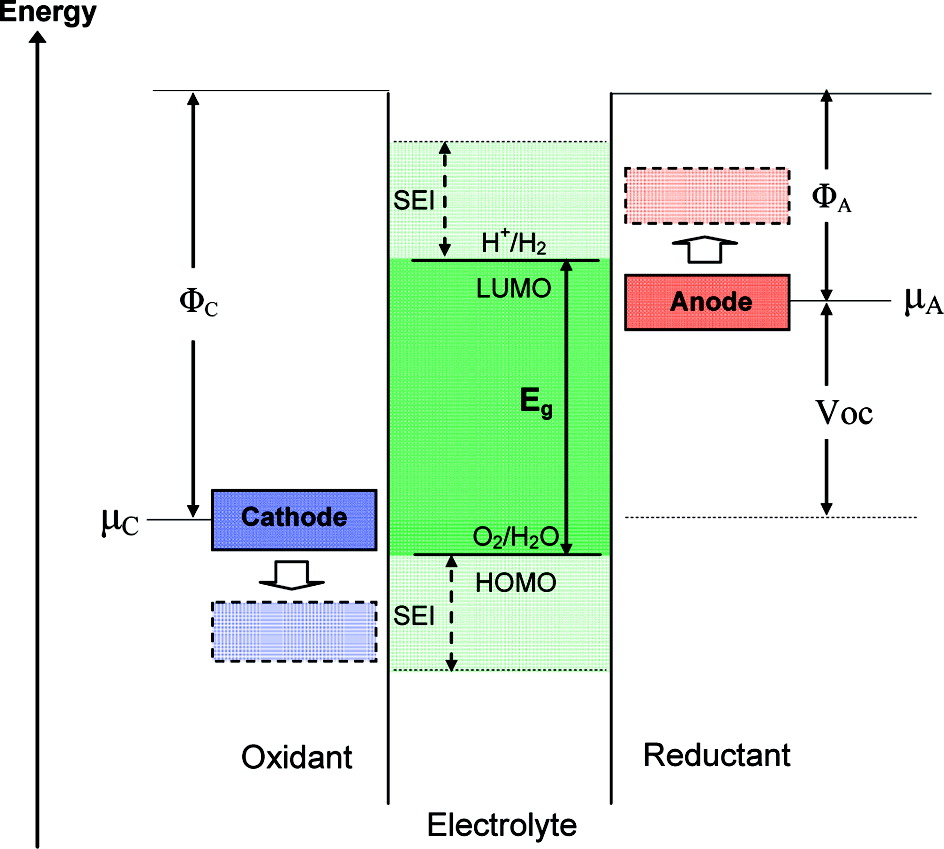
\includegraphics{figures/electrolyte.jpeg}
    \caption{Schematic open-circuit energy diagram of an aqueous electrolyte. $\Phi_{A}$ and $\Phi_{C}$ are the anode and cathode work functions. $E_{g}$ is the electrochemical stability window of the electrolyte. If $\mu_{A}>$ LUMO and/or $\mu_{C}<$ HOMO the electrolyte would be thermodynamically unstable and its usage would require kinetic stability through the formation of a SEI layer. Reprinted with permission from Ref.~\citenum{Goodenough2010}. Copyright 2010 American Chemical Society.}
    \label{fig:electrolyte}
\end{figure}

The energy gap, $E_g$, for an aqueous electrolyte is $\sim 1.3$ eV which severely limits the open circuit voltage, $V_{oc}$. In order to obtain a higher open circuit voltage $V_{oc}$, non-aqueous electrolytes with larger $E_g$ have been used in Li-ion batteries.\cite{Xu2004, Goodenough2010} A good summary of electrochemical stability windows of different classes of non-aqueous electrolytes including (organic and inorganic) liquids, solids, ionic liquids, polymers and their combinations, which have been used in Li-ion batteries is presented by \citeauthor{Goodenough2010}.\cite{Goodenough2010} One of the properties for solid electrolytes is that they generally have a larger electrochemical stability window than liquid electrolytes,\cite{Goodenough2010} hence, can be operated within a larger voltage window, allowing the energy density of the battery to be increased.

\textbf{Ionic conductivity} High ionic conductivity ($>10^{-4}$ S cm$^2$) in the electrolyte (liquid or solid) and across the electrode-electrolyte interphase enables a high rate-capability of the overall Li-ion battery.\cite{park2010review,Goodenough2010,Kamaya2011} Generally, the ionic conductivity of liquid electrolytes is higher than that of solid electrolytes. However, new classes of solid materials have been found with ionic conductivity surpassing that of liquids (cf. section~\ref{sec:solid_electrolytes}), known as superionic conductors. While the ionic conductivity in electrolytes is important, it is not the bottleneck in the overall Li-ion diffusion process, as it is several orders of magnitude higher than that in the bulk of electrodes and the electrode-electrolyte interphase.\cite{park2010review}

% Define and highlight differences of electric double layer and stability window for solids and liquids.
\textbf{Electric double layer} During the charging of an electrode in contact with a liquid electrolyte, excess charge develops at the electrode surfaces. This triggers the rearrangement of electrolyte ions in the electrolyte solution to achieve local electroneutrality at the interfacial region. A local electroneutrality at the electrode-electrolyte interface is maintained by accumulation of counter-electrolyte charge near the interface, resulting in the formation of an interfacial charge density perturbation in order to screen the charge at the electrode surface. In the classical system of dilute electrolytes, this is achieved by the formation of a monotonically decaying `double layer'.\cite{Schmickler2010} Several models of the electric double layer in electrochemistry exist, such as Helmholtz, Gouy-Chapman, and Gouy-Chapman-Stern.\cite{Bard2010} Early models were limited in sophistication: the Helmholtz double layer model suggested charge screening by a plane of counter-electrolyte charges near the electrode surface, resembling a capacitor. In contrast, the Gouy-Chapman model screens charge via a diffuse layer of electrolyte ions decaying monotonically to their bulk concentration value where the electric potential will fall to zero. The Gouy-Chapman-Stern model accounted for discrepancies encountered by including both a Helmholtz layer of counter charge as well a diffuse layer of electrolyte ions, as shown schematically in figure~\ref{fig:edl}(a). These continuum models of electrolyte ions are also being integrated with quantum mechanical methods, such as DFT (c.f. section~\ref{sec:dft+cont}). \citeauthor{neutralization-paper} recently implemented such a hybrid quantum-continuum model to achieve electroneutrality in simulations of charged electrochemical interfaces based on a modified Poisson-Boltzmann equation.\cite{neutralization-paper}

At the interface between solid electrolytes and electrodes, a similar decay in charge is observed. However, in this case the charge carrier is the charge vacancy. \citeauthor{Maier_ProgSolStatChem1995} discuss the theory of this decay in detail \cite{Maier_ProgSolStatChem1995} and new continuum models continue to be developed for solid electrolytes\cite{Mebane_CompMaterSci2015,MebaneAndDeSouza_EnergyEnivronSci2015,TongEtAl_JAmCeramSoc2020,Lund_2021}. \citeauthor{Swift2021} present a model for formation of the double layer in solid-solid electrochemical interfaces based on the Poisson-Fermi-Dirac equation. The resulting space charge layer of point defects in a solid electrolyte material is shown schematically in figure~\ref{fig:edl}(b). However, this study only accounts for the effect of correlations between ions by limiting the concentration of defects in the interfacial layer to be below a certain value.

At higher concentrations, screening of electrodes changes markedly in liquids, with a new regime emerging when the Debye screening length is roughly equal value to the ionic diameter. In this regime, charge is screened by means of exponentially damped oscillations of co-ions and counter-ions, in an ordered interfacial structure known as overscreening\cite{bazant2011double}, a structure that has been previously been observed experimentally for liquids\cite{perkin_ionic_2012, groves2021surface, bowers2004surface, sloutskin2005surface}. This year \citeauthor{dean2021overscreening} became the first to propose the existence of a similar oscillatory decay at solid electrolyte grain boundaries. \cite{dean2021overscreening}

\begin{figure}
    \centering
    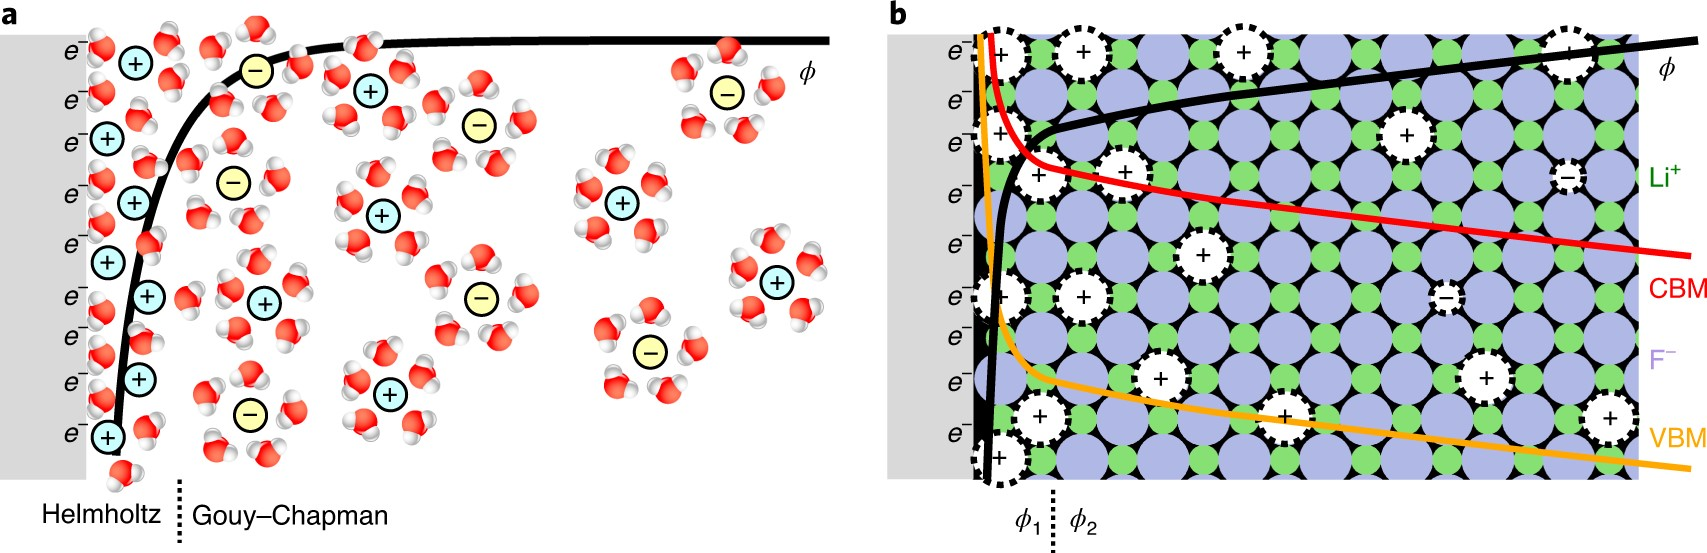
\includegraphics[scale=0.35]{figures/edl.jpg}
    \caption{Schematic comparing the double layer formed at the solid–liquid and solid–solid electrochemical interfaces. (a) For the solid–liquid interface, excess electrons on the electrode are balanced by increased density of solvated positive ions in the liquid electrolyte. $\phi$ is the electrostatic potential, and is mediated by the Helmholtz layer, followed by exponential decay in the diffuse layer (described by Gouy–Chapman theory). (b) For the solid–solid interface, excess electrons on the electrode are balanced by increased density of positive point defects in the solid electrolyte. Electronic band bending must be taken into account in the solid electrolyte. $\phi_1$ and $\phi_2$ are the electrostatic potentials next to and further from the interface. Electronic band-bending is shown via the valence-band maximum (VBM), also known as the HOMO, and conduction-band minimum (CBM), also known as the LUMO. Reproduced with permission from Springer Nature: Ref.~\citenum{Swift2021}, Copyright 2021.}
    \label{fig:edl}
\end{figure}

\textbf{Solid-electrolyte interphase (SEI)} The ``interface'' described above is basically a two-dimensional surface between the electrode and electrolyte. In Li-ion batteries, the electrolyte reacts irreversibly and decomposes on the surface of electrodes leading to the formation of a several nanometers-thick distinct phase between the electrode and electrolyte, known as the solid electrolyte interphase (SEI).\cite{Xu2011} The ability to form a stable interphase at the electrodes, which is also ionically conducting but electronically insulating, is an important criterion for the selection of an electrolyte material. The electron insulating property of the SEI is important to stop further decomposition of the electrolyte on the electrode.\cite{Xu2004,Goodenough2010} High ionic conductivity in the SEI is important for the overall rate capability of Li-ion batteries and often the ionic conductivity in the interphase has been found to be a bottleneck.\cite{Wang2018, Xu2014} While the SEI was originally discovered in the case of liquid-electrolytes, its rate-limiting behaviour is now also observed in all-solid-state batteries.\cite{Yu2017}

The two major classes of electrolyte materials, solid and liquid electrolytes, are discussed separately. We focus on the atomistic modelling of different types of liquid and solid electrolytes, and their battery related properties. For the liquid electrolyte section, this includes the bulk structure, diffusion properties, solvation energies, and activity coefficients of different solvents. For the solid electrolyte section, there is a particular emphasis on the ion transport mechanisms, material stability, and the electrode-electrolyte interfaces. Finally, we discuss the individual challenges and outlook for future atomistic modelling investigations of both liquid and solid electrolytes.

\subsection{Liquid Electrolytes}
\label{sec:Liquid_electrolytes}
\subsubsection{Introduction to liquid electrolyte materials}
The most widely used liquid electrolyte in Li-ion batteries is LiPF$_6$ in a solvent, which is typically a mix of two or more solvents, for example propylene carbonate (PC), ethylene carbonate (EC), ethyl methyl carbonate (EMC), dimethyl carbonate (DMC), in order to achieve competing objectives such as ability to dissolve high concentration of salt, low viscosity, high dielectric constant, at typical operational temperatures.\cite{Xu2004,Xu2014, Logan2020, Valo_en_2005,TARASCON19931221} Cyclic carbonates (EC, PC) have higher dielectric constant but also high viscosity, while ``linear'' carbonates (DMC, EMC) have low viscosity but also low dielectric constant; for that reason often mixtures of solvents are used to optimise performance in a specific application.\cite{Logan2020,Yamada_2013,TARASCON19931221} However, continued innovation in electrolyte mixtures continues to take place. In the last two decades there has been interest in other electrolytes such as ionic liquids\cite{macfarlane2014energy} and salt in water based systems\cite{suo2016advanced}. This section will touch on both the traditional and emergent electrolyte solvents.

\subsubsection{An introduction to modelling liquid electrolytes (Sam/Lucy)}
The modelling of liquid electrolytes for conventional batteries is a broad and diverse field. Over the past 20-30 years atomistic modelling has helped shape the fundamental physics of liquids, determining a new physical basis and validating decades-old pen and paper theories of concentrated electrolytes. \cite{qian2015high,kim2015situ,zhou2009atomistic,enderby1981structure} The development of liquid electrolytes can be presented from an applications approach or a methods approach. Here, we focus on the development of liquid electrolyte models and the considerations needed when modelling these materials, before moving on to their applications in measuring different properties.

Atomistic modelling of liquid electrolytes can be broadly separated into \textit{ab initio} (\textit{First Principles}) and classical (potentials-based) Molecular Dynamics (MD) modelling (c.f. section~\ref{sec:molecular_dynamics}). These are complementary techniques which can be used to aid the other. For example, \textit{First Principles} calculations are able to provide information on the electron distribution, which is required for parameterising the non-bonded components of force fields used in classical MD. Classical MD can also be used to provide the starting conditions for DFT calculations. \textit{Ab initio} and classical methods can also be combined in quantum mechanics/molecular mechanics (QM/MM) studies, where the larger system is treated classically with a smaller sub-region being modelled using \textit{ab initio} methods. For example, a study by \citeauthor{Fujie_2018} used the ``Red Moon'' method to investigate the formation of the solid-electrolyte interface (SEI) at the metallic electrode\cite{Fujie_2018}.

In this section, we first discuss the separate design and use of \textit{ab initio} and classical MD methods, followed by their application for investigating properties in the bulk liquid electrolyte. Finally, we discuss the application of atomistic methods for investigating the solid-electrolyte interface (SEI) from the perspective of the liquid electrolyte (complementary to the solid focused SEI discussion given in section~\ref{sec:SEI}).

\subsubsection{\textit{Ab initio} modelling of liquid electrolytes (Sam/Lucy)}
\textit{Ab initio} calculations on liquid electrolytes provide critical information that can be used to explain their behaviour in experimental applications. For many years DFT calculations (c.f. section~\ref{sec:dft}) have been used to provide information on the electrochemical stability of solvents\cite{Koch_1996}. However, this method was further developed in 2011 when \citeauthor{ong2011electrochemical} used a combined MD and DFT approach to model the electrochemical stability window of several ionic liquids with a higher degree of accuracy than previously seen\cite{ong2011electrochemical}. This methodology has since been widely used in studying the stability of various ions in solution with many key studies being based on the initial work of \citeauthor{vuilleumier2001electronic}\cite{vuilleumier2001electronic}. Here, the authors modelled the ionisation of of sodium and silver ions using \textit{ab initio} MD, which was later extended to model fluctuations in the coordination shells\cite{blumberger2006diabatic}, and then to model copper\cite{blumberger2004electronic} ions and the redox of molecular species\cite{vandevondele2006solvent}. However, the applicability of any such method is somewhat solvent dependent. A point which was made clear by \citeauthor{lynden2007can} on the subject of the difficulties of applying Marcus theory to ionic liquids, where long range electrostatic interactions may become important\cite{lynden2007can}.

\textit{Ab initio} modelling using DFT provides a parameter-free approach to simulate the properties of liquid electrolytes. For example, \citeauthor{Ganesh2011} demonstrated use of \textit{ab initio} MD of liquid electrolytes using the PBE-GGA exchange-correlation functional to calculate the statistical and dynamic properties.\cite{Ganesh2011} They performed simulations of LiPF$_6$ at 310 K and 400 K in EC and PC at densities comparable with typical experimental compositions. They observed a spontaneous decomposition of LiPF$_6$ into Li$^+$ and PF$_6^-$ and a coordination number of 4 for solvated Li$^+$, similar to experiments. The plots of the radial-distribution function of Li-ion with carbonyl oxygen of EC and PC are shown in Figure~\ref{fig:leaimda}. The Li-O (carbonyl) near-neighbour distance in PC is found to be $\sim$1.94~\AA \ at 310 K and $\sim$1.90~\AA \ at 400 K, quite close to the experimentally measured distance of $\sim$2.04~\AA \ by time of flight neutron scattering experiments.\cite{Kameda2007} The  Li-O (carbonyl) peak for EC is $\sim$1.92~\AA \ at 310 K and $\sim$1.90~\AA \ at 400 K which is quite close to that for PC. Comparatively, a classical MD simulation predicted a Li-O (carbonyl) peak $\sim$1.70~\AA.\cite{soetens_molecular_1998} The Li-O=C bond angle distribution is shown in the inset of Figure~\ref{fig:leaimda}. The center of the distribution for PC is at 140$^\circ$ which is in agreement with the experimentally measured value of 138$^\circ$.\cite{Kameda2007} Here, the distribution for EC is predicted to be similar to PC. Calculations using classical MD simulation also predict EC and PC to have similar distributions, though at a much higher Li-O=C angle $\sim$160$^\circ$ for both solvents.\cite{soetens_molecular_1998}

\begin{figure}
    \centering
    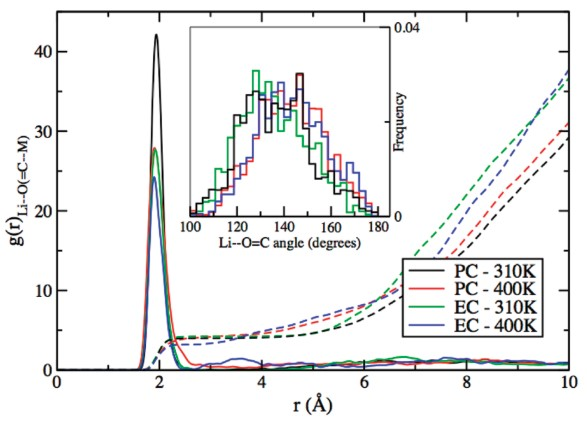
\includegraphics[scale=0.5]{figures/aimda.jpg}
    \caption{Partial radial-distribution function of Li-ion with the carbonyl oxygen of EC and PC along with the partial-density weighted integral (dashed lines) which equals the Li-ion coordination number. In both electrolytes, the Li-O(carbonyl) distance is $\rm \sim2~\AA$ and the first-solvation shell of Li-ion has 4 EC or PC molecules consistent with the experiments. The inset shows the histogram of the Li-O=C angle. Reprinted with permission from Ref.~\citenum{Ganesh2011}. Copyright 2011 American Chemical Society.}
    \label{fig:leaimda}
\end{figure}

Perhaps the most enticing possibility regarding \textit{ab initio} methods at interfaces is to study the liquid-electrode interfacial behavior. The physics of such a study are however complex and therefore trade offs in functional choice and solvent model may need to be made in order to make calculations feasible. \citeauthor{lespes2015using} used an implicit solvent model in order to study the interfacial electrochemistry of lithium ethylene carbonate solutions\cite{lespes2015using}.

While \textit{ab initio} molecular dynamics is free from the effects of arbitrary parameters and highly accurate, a major limitation of this approach is the feasible time and length scales reachable due to high computational cost; generally being restricted to between hundreds (conventional DFT) and thousands of atoms (linear-scaling DFT approaches, c.f. section~\ref{sec:lsdft}) and tens of pico-seconds. The limited time and length scales both introduce inaccuracies and irregularities in the calculations. 

When considering the impacts of small length scales (box size), the critical issue is the introduction of spurious long to medium range correlations of atoms and molecules. As liquids do not exhibit long range order, the presence of periodic images that are located at exactly a cell width in all direction introduces an unphysical correlation. This is observed in the modelling of systematically disordered solids in smaller cells\cite{Morgan_2011}. For example, \citeauthor{Zhao_2020} recently revealed there is a distribution of different low-symmetry local motifs in cubic halide perovskites, such as tilting and rotations, which are only observed if you allow for a larger-than-minimal cell size \cite{Zhao_2020}. Beyond truncating the radial distribution function (RDF) to a shorter distance (i.e. half the shortest distance between periodic images) than is optimal, this effect will also introduce (normally small) inaccuracies in thermodynamic and dynamic quantities\cite{Binder2009book, yeh_system-size_2004, botan_diffusion_2015, horbach_finite_1996}. These inaccuracies are of a particular concern in liquid electrolytes as the electrostatic interactions between ions gives rise to longer range interactions even when the Debye length is far smaller than the box size\cite{coles_correlation_2020}.

In the case of the short time scale of \textit{ab initio} simulations can, particularly for more viscous liquids, lead to highly non-ergodic (fully-sampled) simulations. When snapshots throughout the whole trajectory are highly correlated\cite{frenkel_understanding_2002}, this can lead to problems for both dynamic and equilibrium studies. 

Neither the issue of time correlation or finite size effects has a significant detrimental to the results of \textit{ab initio} studies. However, in specific studies where they need to be avoided, or where a quantum description of a liquid electrolyte provides no significant advantage over a classical description, it is beneficial to turn towards far less computationally expensive (and thus larger and longer) potentials-based simulations.

\subsubsection{Classical modelling of liquid electrolytes (Sam/Lucy)}
\label{sec:electrolyte_classicMD}
Classical simulation of liquid electrolytes includes classical force field based molecular dynamics (c.f. section~\ref{sec:molecular_dynamics}) and the related field of classical Monte Carlo (c.f. section~\ref{sec:monte_carlo}). Classical MD, also known in solid-state communities as potentials-based MD, is a broad field which uses many different types of force fields for different studies. The development of force fields for ionic solids is described in section~\ref{sec:potential_fitting}, whereas here we evaluate the force fields used for liquid electrolytes and the considerations need to develop them. Historically, force fields for different electrolyte systems have developed at similar paces. Here, we use the example of the development of force fields for ionic liquid.

Electrolyte solvents from water, to molecular solvents and ionic liquids, pose a challenge that is not normally present in the solid state, specifically the need to model covalent bonding. This is achieved by splitting the potential acting on each atom into bonding and non-bonding contributions. The non-bonding component accounts for the effects of electrostatics, dispersion, and degeneracy pressure; and the bonding component accounts for the effects of covalent bonding. In classical modelling of liquid electrolytes, we are mainly interested in the behaviour within the electrolyte's electrochemical stability window (c.f. section~\ref{sec:electrolytes_introduction}). Therefore, the vast majority of classical studies model bonds with unbreakable, harmonic potentials. There are four distinct types of bonded potential \cite{lindahl_gromacs_2021, frenkel_understanding_2002}: bonds, angles, dihedrals, and improper dihedrals. These can be traced back to the parameterisation of force fields, such as OPLSA-AA\cite{canongia_lopes_clp_2012, jorgensen_development_1996}, and are often parameterised from spectroscopic force constants. There are many ways of defining bonded potential types in available codes\cite{lindahl_gromacs_2021,PLIMPTON19951}, though their discussion is beyond the scope of this review. Atoms which are subject to a bonded potential are often wholly, or partially, excluded from non-bonded interactions, though in large molecules non-bonded intramolecular interactions are important. Alternatively bonds can be kept rigid using a constraint algorithm\cite{hess_lincs_1997,ryckaert_numerical_1977,andersen_rattle_1983}.

When developing force fields, generally, it is the non-bonded force field components, in particular the partial charges on atoms, which are more frequently varied. A common model for liquids electrolytes is the OPLS-AA force field.\cite{jorgensen_development_1996} This is a Lennard-Jones potential based force field with an additional coulombic term. \cite{ewald_berechnung_1921,darden_particle_1993,deserno_how_1998,yeh_ewald_1999}.

Further developments can be made from this base force field, such as the CP\&P force field \cite{canongia_lopes_clp_2012, canongia_lopes_modeling_2004, canongia_lopes_molecular_2004, canongia_lopes_molecular_2006} which describes a wide range of ionic liquid cations and anions. Some non-bonded parameters, particularly charges, were varied from OPLS-AA. The charges on the individual molecules are obtained form \textit{First Principles} calculations (DFT), in this case by use of the charge mapping algorithm CHelpG\cite{canongia_lopes_clp_2012} (though other algorithms may also be used\cite{spackman_potential_1996,breneman_determining_1990,singh_approach_1984}). 

Electrostatic interactions are important when modelling charged electrolytes, as are the effects of polarisability. Often it is advantageous in a non-polarisable force field to scale the charge on each ion down from a value of 1$e$\cite{schroder_comparing_2012, schroder_polarizable_2020, shimizu_structural_2015}. This accounts for the effect of polarisability on the strength of electrostatic interactions between ions, which is particularly important for transport properties. However, other force fields have been defined to account directly for polarisability \cite{schroder_polarizable_2020}. As described in section~\ref{sec:potential_fitting}, polarisability can be introduced to a force field by the employment of Drude Oscillators (core shell model) \cite{schroder_polarizable_2020, schroder_comparing_2012, lindahl_gromacs_2021}. This approach is computationally cheap and is core to the polarisable ionic liquid force field developed from CL\&P by \citeauthor{schroder_comparing_2012} \cite{schroder_comparing_2012}. A more advanced representation of polarisability can be provided by an intrinsically polarisable force fields, normally based on the Fumi-Tosi potential. \cite{sangster1976interionic} This method has been used for molten salts \cite{madden_covalent_1996}, ionic liquids \cite{borodin_polarizable_2009, schroder_polarizable_2020}, and lithium salts in molecular solvents \cite{borodin_litfsi_2006,bedrov_molecular_2019,bedrov_influence_2010}. This provides the best description of polarisability in a classical force field, however, there is an associated higher computational cost, and often require a particular code to implement (such as metalwalls \cite{marin-lafleche_metalwalls_2020}).

The development of force fields for metal cations has seen an equal level of discussion and interest. These cations can be slightly easier to model computationally owing to their relative non-polarisability \cite{mamatkulov_force_2013,mamatkulov_force_2018,schroder_polarizable_2020}. They are frequently modeled as Lennard-Jones spheres to match the potential in the prevailing solvent models (SPC and OPLS-AA). For alkali and alkali earth metal cations a wide range of values of $\sigma$ (excluded volume) and $\epsilon$ (interaction strength) can be used as the basic energetics associated with one of these force fields can be recovered for many pairs of sigma and epsilon values. The choice of which pair of parameters to use is normally driven by which property you are most interested in accurately reproducing \cite{mamatkulov_force_2013}. It is worth noting that many force fields used to modeled the electrolytes of specific interest to us here, were parameterised for aqueous solutions\cite{mamatkulov_force_2013}.

\subsubsection{Bulk Structure and Landscaping (Sam/Lucy)}
%Bulk structure and landscaping(?)
For structural analysis of liquid electrolytes, analysis of the radial distribution function (RDF) is the mostly widely used approach. RDFs can be converted to structure factors by a simple Fourier transform into reciprocal space, allowing for easy comparison with experimental structure factors\cite{shimizu_structural_2015, pethes_comparison_2017, hanke_intermolecular_2001,tsuzuki_molecular_2009}, subject to re-scaling for the specific intensities associated with different atoms. This method has been frequently used for a broad array of electrolytes, and has seen particular utility for ionic liquids, where the large inhomogenous ion surface can lead to complex patterns for which molecular dynamics can provide explanation. Modelling of this sort of behaviour has been performed for aprotic\cite{Migliorati_2015} solvate ionic liquids\cite{shimizu_structural_2015}, imidazolium salts\cite{hanke_intermolecular_2001}, lithium carbonate solutions\cite{Chaudhari_2018} and highly concentrated aqueous solvents\cite{pethes_comparison_2017}.

The physical relevance of RDFs does actually go further than this; however, the RDF is closely related to potential of mean force acting on a particle. This describes the changing potential landscape acting between particles as they approach one another\cite{frenkel_understanding_2002}. As well as being generated from a RDF, the potential of mean force can be obtained by direct calculation by use of centre of mass pulling, umbrella sampling\cite{lindahl_gromacs_2021}, or running multiple calculations with ions frozen an exact distance apart from one and other. When modelling liquid electrolytes this method is also used to study the approach of ions to an electrode where the energetics associate with decoordination from the solvent and coordination to the electrode can be modelled. For example, \citeauthor{sergeev_electrodeelectrolyte_2017} looked at the approach of oxygen and lithium based species towards electrodes\cite{sergeev_electrodeelectrolyte_2017}. Here, the authors performed MD simulations of the electrode/electrolyte interfaces of a Li-O$_2$ cathode under potentials close to experimental values in 1 M dimethyl sulfoxide (DMSO) solution of LiPF$_6$ salt. They find that oxygen anions are effectively pushed out of the reaction layer, making the second reduction of superoxide anion hardly probable, indicating the main cause of the electrode surface passivation is the presence of lithium superoxide near the electrode surface. \citeauthor{sergeev_electrodeelectrolyte_2017} proposes that a way of suppressing the passivation is to shift the equilibrium \.{O}$_{2}^{–}$ + Li$^+ \rightleftharpoons$ LiO$_2$ to the side of separately solvated ions, for example, by using solvents resulting in lower free energy of the ions. \cite{sergeev_electrodeelectrolyte_2017}

\subsubsection{Li-ion Diffusion (Sam/Lucy/Arihant)}
%Diffusion
Diffusion (c.f. section~\ref{sec:diffusion}) plays a critical role in the operation of liquid electrolytes through its impact on conductivity. However, in liquid electrolytes its impact goes deeper as the dielectric constant of liquids consists of both dipolar and ionic contributions. These two contributions can be obtained by analysis of the dipole orientation and current auto-correlation functions using the Einstein-Helfand method. For example, \citeauthor{coles_correlation_2020} performed this analysis on four liquid electrolytes (three in aqueous solvent and one in a common organic solvent mixture): aqueous solutions of LiCl, NaI, and LiTFSI, as well as the same LiTFSI salt solvated in an equimolar mixture of DME and DOL \cite{coles_correlation_2020}. Here, it was shown that for polar solvents the dipolar contribution is nearly always dominant, with current acting as correction which could feasibly be neglected (particularly for more dilute systems). For ionic liquids, which contain ionic species that can exhibit a net dipole, such as bistriflimide, both dipolar and ionic contributions would be observed. The effect of molecular ions having simultaneous charges and dipoles was explored by \citeauthor{schroder_collective_2011} who showed even more thorough treatment may be required to observed the impacts of their interplay\cite{schroder_dielectric_2009}.

The self-diffusion coefficient can be calculated from the slope of the mean-squared displacement, according to the Stokes-Einstein relation. For example, \citeauthor{Ganesh2011} calculated the mean-squared displacement of solvated Li-ion in EC and PC solvents from \textit{ab intio} MD as shown in Figure~\ref{fig:leaimdb}. For PC, the self-diffusion coefficient is calculated to be $\sim0.7\times10^{-9}$ m$^2$ s$^{-1}$ at 310 K while the experimentally measured value of self-diffusion coefficient at 303 K is $\sim0.16\times10^{-9}$ m$^2$ s$^{-1}$.\cite{Hayamizu1999}. For EC, it is calculated to be $\sim1.0\times10^{-9}$ m$^2$ s$^{-1}$ at 310 K while the experimentally measured value of self-diffusion coefficient at 313 K is $\sim0.21\times10^{-9}$ m$^2$ s$^{-1}$.\cite{Hayamizu1999}. At 400 K, the calculated diffusion coefficient for PC increases to $\sim3.7\times10^{-9}$ m$^2$ s$^{-1}$, while it remains the same for EC. It is notable here that the Li-ion diffusion in the electrolyte solution is 4-5 orders of magnitude higher than that in the bulk of electrodes e.g. graphite anode (cf. section~\ref{sec:anodes_ion_diffusion}).

\begin{figure}
    \centering
    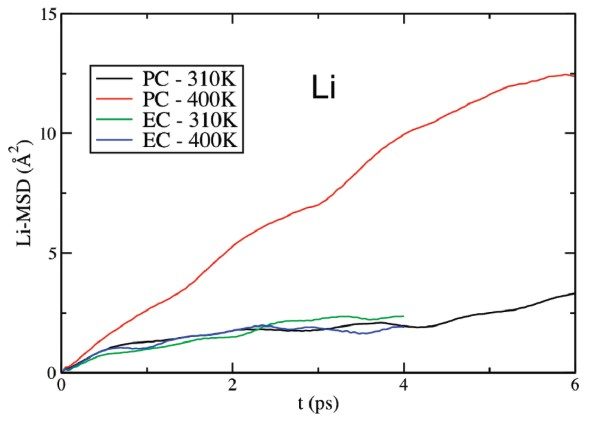
\includegraphics[scale=0.5]{figures/aimdb.jpg}
    \caption{Mean-squared displacement of solvated Li-ion in EC and PC. Reprinted with permission from Ref.~\citenum{Ganesh2011}. Copyright 2011 American Chemical Society.}
    \label{fig:leaimdb}
\end{figure}

Investigation of the diffusion of different ions subject to a field gives a sense of the diffusion rate of specific ions and also an idea of exchange rates of solvent molecules. Strongly coordinated solvents will have diffusion coefficients closer to the ions they are coordinated to than less strongly coordinating ligands \cite{shimizu_structural_2015, lesch_influence_2015, borodin_litfsi_2006,borodin_li_2006,borodin_li_2007}. Examples of this behaviour can be found in the molecular dynamics studies of \citeauthor{borodin_li_2006} which looked at diffusion in lithium solutions of both the common carbonate\cite{borodin_litfsi_2006} and elthylene glycol oligomer solvents\cite{borodin_li_2006}. For the common carbonate, MD predictions of the ion and solvent self-diffusion coefficients and conductivity were in good agreement with experiments, with approximately half of the charge transported by charged ion aggregates with the other half carried by free ions.\cite{borodin_litfsi_2006} The self-diffusion coefficients and conductivity predicted by MD for the ethylene glycol oligomer solvents were also found to be in good agreement with experimental data. Li$^+$ transport was found to primarily occur though exchange of TFSI$^-$ anions in the first coordination shell.\cite{borodin_li_2006} The 2015 study of \citeauthor{shimizu_structural_2015} investigated a number of different lithium glyme solvate ionic liquids\cite{shimizu_structural_2015}. Here, the authors found that although MD was unable to yield quantitative information about the dynamics of the system, it could provide two important pieces of information: the auto-diffusion coefficients of glyme molecules in pure glyme are much larger that those of glyme molecules in glyme equimolar mixtures at the same temperature; the decrease in the glyme diffusion coefficients is more pronounced in the Li[Ntf$_2$] + glyme system than in the Li[NO$_3$] + glyme mixture.\cite{shimizu_structural_2015} The study of \citeauthor{lesch_influence_2015} used MD to investigate lithium salts dissolved in aprotic ionic liquids.\cite{lesch_influence_2015} The authors found that the exchange of TFSI anions in and out of the first coordination shell of Li$^+$ was faster in pyr$_{13}$-based systems compared to emim-based systems, and the Li$^+$ ion transference number to be higher. \cite{lesch_influence_2015}

In more complex solvents such as ionic liquids the nature of solvent plays a important role too, for instance \citeauthor{borodin_li_2007} showed the effect of flouriation of ionic liquid cations on diffusion behaviour\cite{borodin_li_2007}. This sort of study can be directly contrasted with pulsed field gradient nuclear magnetic radiation (NMR) experiments of the type normally used to study battery materials. This was done, for example, when \citeauthor{shimizu_structural_2015} studied lithium bistriflimide based solvate ionic liquid which had been proposed as a solvent for Lithium Sulfur batteries \cite{shimizu_structural_2015}.

\subsubsection{Solvation Energies (Sam/Lucy)}
%Solvation energies
Solvation energies in electrolytes have been widely studied and though research focus has been on aqueous solvation of biomolecules, these techniques can also be used to look at solvation of metal ions with organic solvents. Dependent on the exact thermodynamics of the system, the solvation energies of ions may be obtained by a number of methods. \citeauthor{Skarmoutsos_2015} used joint DFT and MD methods to look at the solvation structures of lithium salts in ternary mixtures of different carbonate solvents. \cite{Skarmoutsos_2015} \citeauthor{Skarmoutsos_2015} showed that different solvents in the ternary mixture were found to dominate at different distances from a central lithium cation, with a particular preference for solvation of lithium by dimethyl-carbonate ions over propylene carbonate and ethylene carbonate being observed, as shown in Figure~\ref{fig:solvation}. \citeauthor{Takeuchi_2012} looked even deeper at the energetics behind the direct contact between cations and anions in solution\cite{Takeuchi_2012}. The relative stabilities of the mono-, bi-, and tri-dentate coordination structures were assessed with and without solvent, where water, PC, and DMC were found to favour the contact ion-pair (CIP)–solvent contact. Vacant sites of Li$^+$ cation in CIP are solvated with three carbonyl oxygen atoms of PC and DMC solvent molecules, and the solvation is stronger for the monodentate CIP than for the multidentate. \cite{Takeuchi_2012}

These are just a few notable studies on solvation energies in liquid electrolytes. A full theoretical description of solvation is given by \citeauthor{Lazaridis_1998} in Ref.~\citenum{Lazaridis_1998}.

\begin{figure}
    \centering
    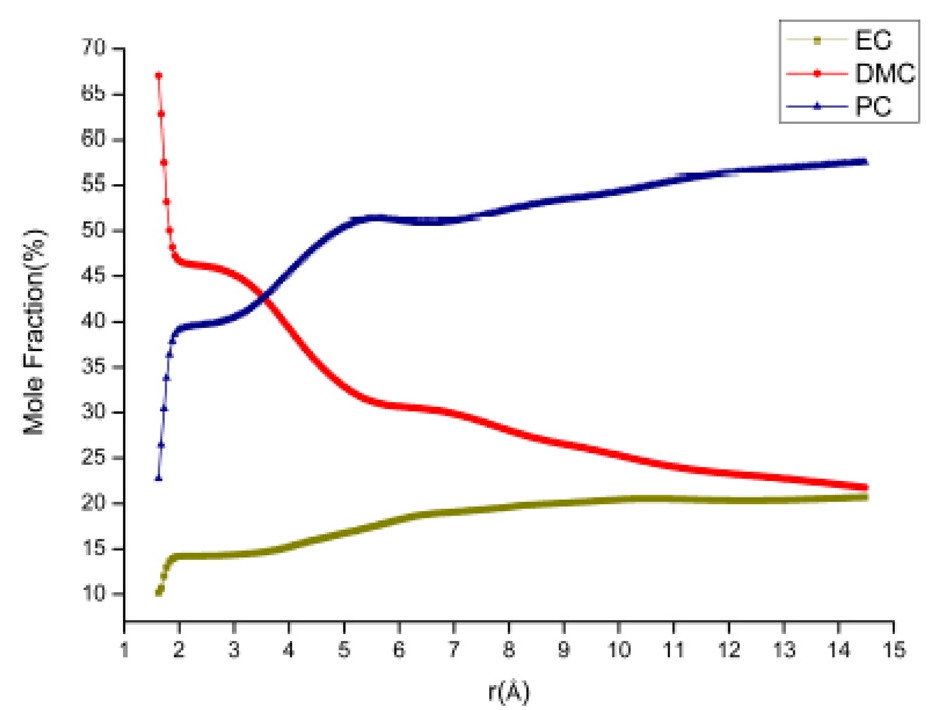
\includegraphics[scale=0.3]{figures/solvents_ternary_mixute_le.jpg}
    \caption{Local mole fractions (\%) of EC, PC, and DMC as a function of the distance from the lithium cation in the ternary mixture. Reprinted with permission from Ref.~\citenum{Skarmoutsos_2015}. Copyright 2015 American Chemical Society.}
    \label{fig:solvation}
\end{figure}

\subsubsection{Activity coefficients of electrolytes (Arihant)}
The activity coefficients describe the deviation of actual electrolytes from an ideal mixture of substances.\cite{Atkins2014} The activity coefficients of electrolyte can be calculated using DFT+P-BE simulations of solutes in electrolyte solutions as described in sec~\ref{sec:tf}. The experimental value of bulk permittivity of ethylene carbonate is ($\veps^\infty=90.7$)\cite{Hall2015} and the surface tension of EC is (0.0506~N m$^{-1}$)\cite{Naejus2002}. These values were used by \citeauthor{Dziedzic2020} to calculate the activity coefficient of LiPF$_6$ in ethylene carbonate (EC) solvent. \cite{Dziedzic2020} The solvent radius was set to $R^\textrm{solvent}_k= 10.5~a_0$ to approximate the size of an EC molecule, and the isovalue of solute electronic density ($\rho_{\textrm{e}}^\lambda$) is varied to match the experimental activity coefficients. A plot of the computed activity coefficients as a function of the square root of electrolyte concentration is given in Figure~\ref{fig:ac}, along with experimental values from Ref.~\citenum{Stewart2008}. Here, we see a good agreement for $\rho_{\textrm{e}}^\lambda=0.002~e/a_0^3$. Trends are also plotted from the linearised approximation of P-BE where the solvent radius is reduced to resemble the prediction for point charges from the Debye-H\"uckel theory.\cite{debye1923theory} The thermodynamic factor can be obtained from numerically differentiating these curves. This is a novel technique of calculating activity coefficients and thermodynamic factors from hybrid atomistic-continuum methods.

\begin{figure}
    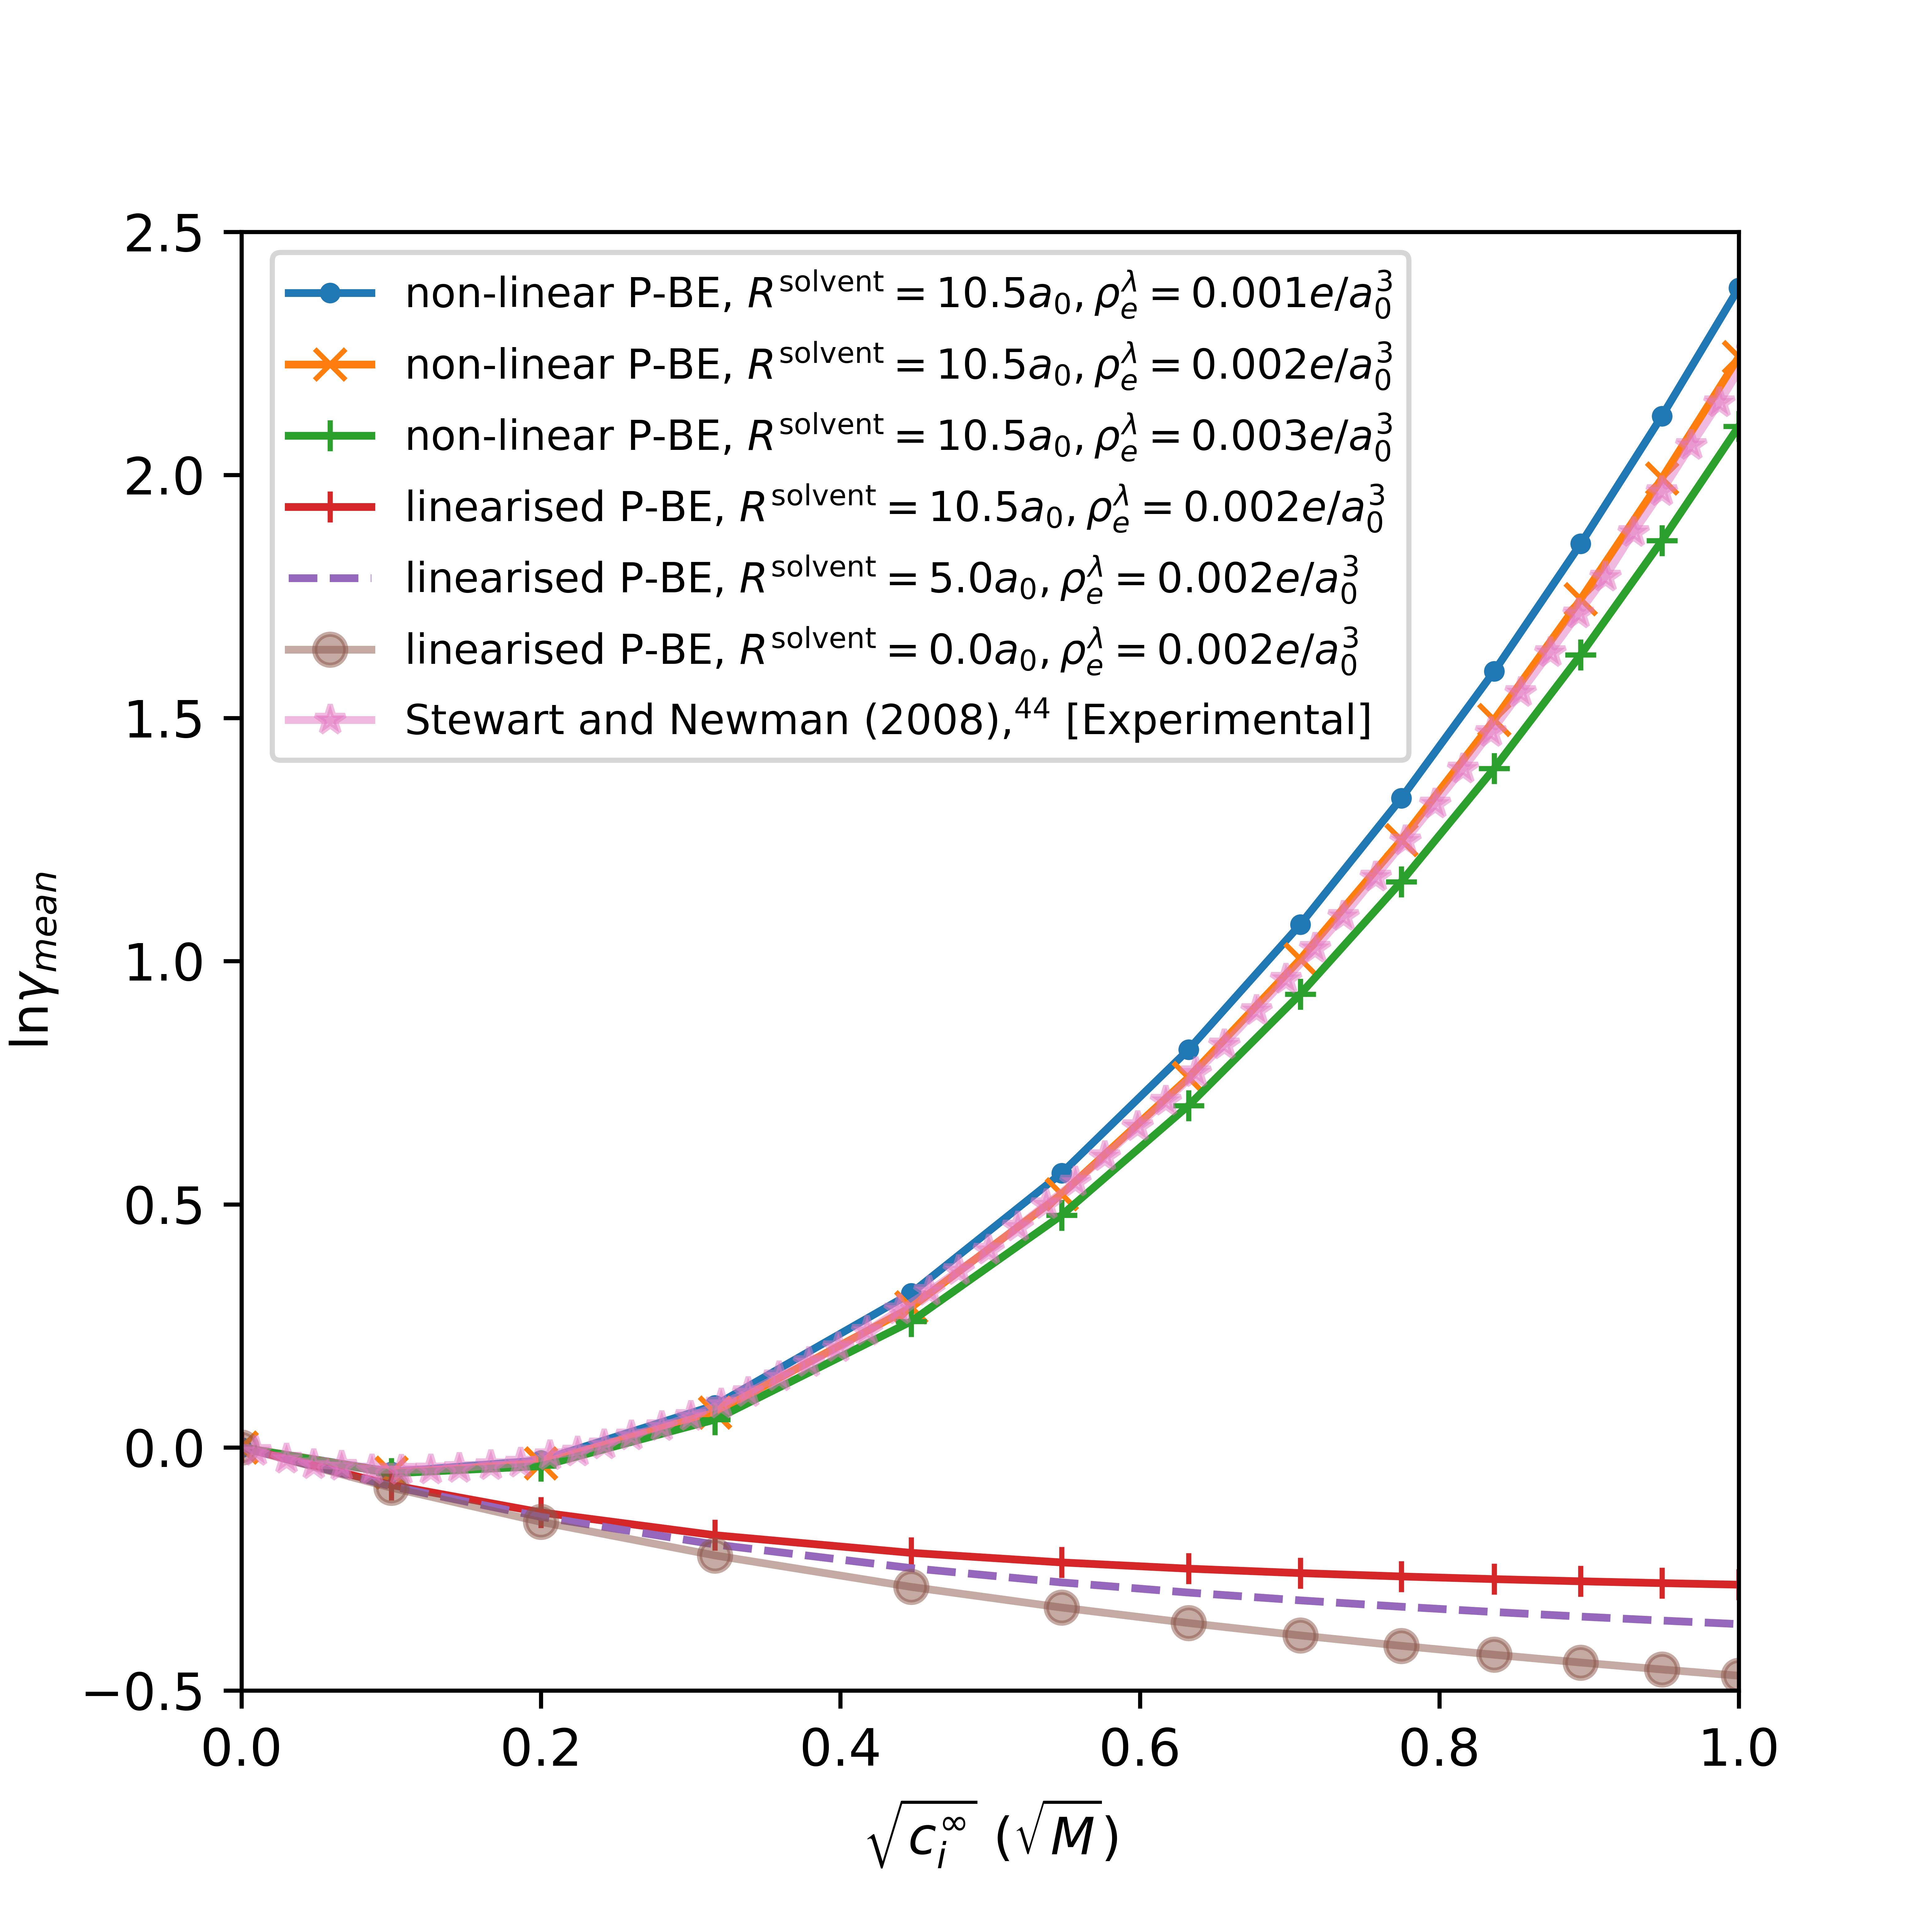
\includegraphics[scale=0.8]{figures/lipf6.png}
    \caption{Mean activity coefficients for LiPF$_6$ in ethylene carbonate at $T=308$~K as a function of concentration and for different values of the atomic electronic density isovalue parameter which determines the extent of the accessibility function. Calculations with the linearised approximation to P-BE are also shown. Reprinted with permission from Ref.~\citenum{Dziedzic2020}. Copyright 2020 American Chemical Society.}
    \label{fig:ac}
\end{figure}

\subsubsection{Interfacial Nanostructure of Electrolytes (Sam/Lucy)}
%Interfaces
In sections \ref{sec:anodes_surfaces_interfaces} and \ref{sec:cathode_interfaces} the interfaces between solids and liquids from the perspective of the solid have been discussed. However, the interface from the perspective of the liquid is also of interest. The structure of liquid electrolytes at metallic\cite{merlet_simulating_2013} and charged dielectric\cite{smith_electrostatic_2016} interfaces will normally extend away from the interface region and can be observed prominently for tens of nanometers, and dependent on concentration of the liquid can either be monotonic or oscillatory as describe in section~\ref{sec:Liquid_electrolytes}.

Concentrated electrolytes and ionic liquids both adopt the characteristic overscreening structure at charged interfaces, including electrodes. This structure, comprising oscillations of charge decaying into the bulk, is commonly observed\cite{coles_nanostructure_2017, merlet_simulating_2013}. Modelling these systems requires an appropriated electrode model. While interesting information can be gained from simulating ions at an electrode with a fixed charge, for example in a high throughput study looking at structural changes with electrode surface charge\cite{coles_nanostructure_2017}, fixed potential boundary conditions will provide a more accurate description of the capacitance \cite{merlet_simulating_2013, scalfi_semiclassical_2020}, interfacial structuring of a liquid electrolyte \cite{coles_simulation_2019, vatamanu_ramifications_2017, li_capacitive_2018}, and the decoordination and dechelation dynamics of coordinated ions\cite{vatamanu_molecular_2009}. Though we note that in light of a recent study by \citeauthor{scalfi_semiclassical_2020} this field continues to evolve as more and more nuanced classical electrode models are employed, such as the Thomas-Fermi based model proposed by \citeauthor{scalfi_semiclassical_2020}. \cite{scalfi_semiclassical_2020}

A wide variety of different electrolytes have been studied using fixed potential electrolytes, from ionic liquids to concentrated electrolyte. Both nanoporous \cite{merlet_highly_2013, merlet_molecular_2012, vatamanu_molecular_2009, vatamanu_ramifications_2017} and nanoscopically rough electrode surfaces have been heavily used\cite{vatamanu_influence_2011}. A specific example of interest is the work of \citeauthor{borodin_interfacial_2014}, where MD simulations were performed on dilithium ethylene dicarbonate (Li$_2$EDC) and dilithium butylene dicarbonate (Li$_2$BDC) in contact with mixed solvent electrolyte (EC:DMC) doped with LiPF$_6$. \cite{borodin_interfacial_2014} In this study the authors examined the SEI–electrolyte interface and found an increase of EC and PF6$^{–}$ molecules and a decrease of DMC at the interfacial layer next to the SEI surface compared to bulk electrolyte concentrations. The activation energies for the Li$^{+}$ solvation–desolvation reaction were estimated to be 0.42--0.46 eV for the Li$_2$EDC–electrolyte and Li$_2$BDC–electrolyte interfaces.
    
\subsubsection{Outlook and challenges (Julian/Arihant/Sam/Lucy)}
% Add a lead in couple of sentences like the other outlooks.
Liquid electrolytes will likely remain the most prominent form of commercialised electrolyte for battery applications in the near future. This is partly due to their monopoly in the market, and partly due to their low cost, which will continue to drive popularity. Despite the overwhelming success of commercialising liquid electrolytes, there is still room for further performance improvements, with several key issues as limiting factors. Liquid electrolytes are known to be limited by narrow electrochemical windows, solvent toxicity, and material flammability/safety concerns. There are two potential avenues for solving these issues:
\begin{itemize}
    % new families of liquid electrolytes to resolve safety issues (Sam)
    \item Resolving these limitations within the confines of liquid electrolytes: ionic liquids have a large electrochemical window, high thermal stability, and their conductivities are similar to those of conventional organic solvent solutions.\cite{macfarlane2014energy} However, they are expensive and there are associated safety concerns.\cite{kralisch2005energetic, smiglak2006combustible} A liquid electrolyte alternative to this could be in water-in-salt electrolytes. Water-in-salt electrolytes are a novel class of electrolytes, which inverts the conventional idea of a salt being dissolved in a solvent, with a small amount of water being dissolved in a hydroscopic lithium salt to the point where a liquid is obtained,\cite{suo2015water,chen2020water} analogous to the high concentration organic electrolyte solutions described by \cite{Yamada_2013}. These liquids have the advantage of being comprised solely of a lithium salt and water, which decreases cost and eliminates safety concerns traditionally associated with organic solvents. The high concentration of salt also leads to a greatly expanded electrochemical window of 3~V \cite{suo2016advanced} from the 1.23~V value for dilute aqueous solutions. However, the highly concentrated solutions in these electrolytes lead to issues of re-crystallisation of the lithium salt, and low conductivity due to the high viscosity of the liquid associated with this concentration of charge carriers\cite{chen2020water,li_transport_2019}.

    %The importance of moving from liquid to solids and the challenges involved. (Safety and energy density).
    \item Replacing liquid electrolytes with solids or soft matter alternatives: despite the success of liquid electrolytes in Li-ion batteries, a number of issues have arisen that may prove impractical to address within the grouping of liquids. Organic liquid electrolytes are highly flammable, leading to safety issues when deployed in portable electronic devices and electric vehicles, such as thermal runaway.\cite{Shepherd_Siddiqui, McCurry_2017, Pfrang2017} Failure modes that cause such safety issues become nearly inevitable occurrences when used by a large volume of people, frequently, as evidenced by electric vehicle and portable device explosions making the news headlines. 
    
    The use of liquid electrolytes also limits the compatibility with electrode materials and thereby limits the maximum energy density of a battery.\cite{Liu2019_e_den} For example, higher energy density Li/S batteries are unstable due to interactions between the liquid electrolyte and the electrodes.\cite{Zhang2013_PS} Similarly, Li metal anodes cannot be used with organic liquid electrolyte solvents without additives\cite{Wu2019_Li_electrolyte} because of dendrite formation and capacity loss.\cite{Kushima2017, Lin2019_li_corrosion} Due to these concerns, research in recent years has shifted to looking at alternatives such as solid and soft matter based electrolytes.\cite{Zhang2018se_review} Solid electrolytes are discussed in detail in the next section (c.f. section~\ref{sec:solid_electrolytes}) and soft matter electrolytes are discussed in detail by \citeauthor{Hallinan_2013} and \citeauthor{popovic2011chemistry}. \cite{Hallinan_2013,popovic2011chemistry}
\end{itemize}
    
% Electrode-electrolyte compatibility
%\item Compatibility between electrolyte types and cathode types. In terms of the cathodes, we discuss layered oxides (NMC), layered oxides (LiMn$_2$O$_4$), and polyanions (LiFePO$_4$), so if we can link electrolytes to these specific materials, it would prelude to the cathodes section. Decomposition of the solvent. 1 sentence on anode and reference section.
The design of the electrode-electrolyte interfaces affects the irreversible capacity loss in Li-ion batteries, and has been found to be a bottleneck in the overall rate capability of the Li-ion battery.\cite{Xu2011,Xu2014} Further work to design better interfaces that are compatible with the electrodes, thermodynamically stable, kinetically fast for Li-ion transfer, electronically insulating, and which lead to minimal loss in performance, will be crucial to progress in Li-ion batteries.\cite{Xu2004, Goodenough2010, Yu2017} Atomistic modelling can help in this area by not only through analyzing chemical reactions that lead to the formation of SEI, but also by predicting new materials enabling a better design of the SEI.\cite{Wang2018} Further details of the interplay between the SEI and graphite anodes are summarised in section~\ref{sec:SEI}.
    
% Modelling challenges
Liquid electrolytes are complex substances, which are difficult to fully capture in atomistic models. In recent years, the computational capacity has expanded to allow for more complex models to be studied. With this, development of new computational methods has allowed research of these complex materials to become more accessible to researchers through freely available open source codes. \cite{merlet_highly_2013, borodin_interfacial_2014, Simoncelli_2018,marin-lafleche_metalwalls_2020}. Future advances in computational ability combined with improved physical studies provide a framework for high throughput screening of electrolyte materials. This could lead to some of the simplest models (such as modelling the interfacial nanostructure of liquids at fixed charge planar electrodes\cite{merlet_simulating_2013}) becoming fairly obsolete.

Developments in expanding the achievable time and length scales of \textit{ab initio} MD will allow more complex models to be developed. However, it is still implausible that \textit{ab initio} MD will be able to applied on large enough systems for long enough that simulations would be fully ergodic (statistically converged) from the perspective of both spatial and time correlations. Therefore, there will remain a space for methods which can provide long scale simulations. In particular, the emergent field looking to fit machine learnt potentials for liquid electrolytes is attractive\cite{shao2021modelling, hellstrom2016concentration, tovey2020dft}. Classical models will likely also be developed, embracing more complex models by incorporating polarisability\cite{marin-lafleche_metalwalls_2020,schroder_polarizable_2020} or bond breaking dynamics\cite{fedkin2019development,hossain2020lithium}. This would then allow for the possibility of modelling electron transfer, bond formation, and the effect of ion and solvent polarisability at larger scales and in greater detail.
    
Atomistic modelling of liquid electrolytes does not necessarily require more computational expense to advance. Work towards exploiting underused physical methods to model liquid systems at far lower cost has been explored. One such method, classical DFT (c.f. section~\ref{sec:dft}), has already been applied to model aqueous capacitors\cite{jeanmairet2019study} and confined ionic liquids\cite{forsman_classical_2011}. This has the potential to be coupled with electronic DFT\cite{jeanmairet2019study} and be used to model electron transfer\cite{jeanmairet2019molecular}.

% Need a brief closing sentence
It should be emphasized that, for practical use, the interfaces between the liquid electrolyte and the electrodes are the major limiting factors in terms of performance, stability, and safety. Therefore, advancement through electrolyte design is crucial. Development of novel electrolyte salts, solvents, or salts is essential for resolving the critical obstacles discussed here. Several articles discuss the challenges of this topic in greater detail. \cite{jie2020advanced,francis2020lithium,xiong2018toward}

\subsection{Solid Electrolytes (Lucy/Julian/Arihant/Rana)}
\label{sec:solid_electrolytes}

\subsubsection{Introduction (Rana/Lucy/Arihant)}
%Brief History of solid electrolytes, types of solid electrolytes, types of properties which are important for batteries. Then which we will focus on in this section sulfides (using LGPS and argyrodites), oxides (Examples), composites (example).
% Possibly we can select some of the below to mention. I think the Van de Ven review covers them all, but we can focus on a few.
% Oxides - NASICONs, LISICONS, perovskites (LLTO), Li garnets, nanocomposites (ranas)
% sulfides - glass ceramics, thio-LISICON (LGPS), argyrodites.
% Others - nitrides, oxynitrides (LiPON), antiperovskites

Solid electrolytes have attracted considerable attention as an alternative to highly-flammable liquid electrolytes, as they significantly improve device safety and have the potential to improve energy and power densities, while also reducing the cost of synthesis. \cite{janek_solid_2016, culver_designing_2018, famprikis_fundamentals_2019, goodenough_li-ion_2013, DIRICAN201927} An ideal solid electrolyte material should possess high electronic resistance, high ionic conductivity, outstanding thermal stability, strong electrochemical stability, excellent mechanical strength, and reduced interfacial resistance. \cite{han2020recent, manthiram2017} There are three different categories of solid electrolytes which are used in rechargeable batteries \cite{DIRICAN201927}: (1) Inorganic ceramic electrolytes, (2) Organic polymer electrolytes, and (3) Composite electrolytes. 

Solid electrolytes were discovered by Michael Faraday in the early 1830s through research on the conduction properties of heated solid sliver sulfide (Ag$_{2}$S) and lead fluoride (PbF$_{2}$) \cite{Faraday1833}.  The use of a ceramic-based $\beta$-alumina (Na$_{2}$O$\cdot$11Al$_{2}$O$_{3}$) in high-temperature sodium-sulfur batteries in the 1960s was considered as a milestone in the development of batteries enabled by solid electrolytes \cite{armand2008building}. In the 1980s the Zeolite Battery Research Africa (ZEBRA) group developed the ``ZEBRA'' batteries using Na$_{2}$O$\cdot$11Al$_{2}$O$_{3}$ as the solid electrolyte. \cite{ZEBRA} So far, the high-temperature sodium–sulfur battery has been commercialised in Japan \cite{oshima2004}, whereas the ZEBRA battery is currently being developed by the General Electric Corporation in the United States. \cite{capasso2014} 

In 1990, the Oak Ridge National Laboratory synthesised a lithium phosphorus oxynitride (LiPON) material \cite{dudney1992,bates1992}, which opened up the use of inorganic solid-state electrolytes in lithium-ion batteries. Since then, a huge number of inorganic lithium-ion conductive ceramic materials have been developed, including perovskite-type \cite{inaguma1993}, garnet-type oxides \cite{kasper1969,mazza1988}, garnet-type sulfides \cite{kennedy1986}, lithium super ionic conductor (LISICON) \cite{ivanov1988}, sodium super ionic conductor (NASICON)-like materials \cite{lang2015}, lithium-argyrodite materials, \cite{deklerk2016} and Li-rich anti-perovskites. \cite{dawson2018elucidating,ahiavi2020mechanochemical}

Despite recent advancement in research activities on crystalline inorganic electrolytes, they are still brittle and therefore difficult to fit into different battery shapes. Solid-state polymer electrolytes (SPEs), due to their high flexibility, can fit in any battery shape and present improved safety and stability features compared to crystalline inorganic electrolytes. \cite{DIRICAN201927} Since 1980, various high-molecular weight dielectric polymer hosts were investigated as polymer electrolytes with high conductivities for lithium batteries, such as poly(ethylene oxide) (PEO) \cite{fenton1973}, polyacrylonitrile (PAN) \cite{abraham1990,dautzenberg1994}, poly(vinylidene fluoride) (PVDF), \cite{arcella1999,kataoka2000,li2016} poly(methyl methacrylate) (PMMA) \cite{appetecchi1995,bohnke1993} and poly(vinylidene fluoride-hexa-fluoropropylene) (PVDF-HFP) \cite{abbrent2001,park2008,yang2014}.

The ionic conductivities of most polymer electrolytes are significantly lower than those of both oxide solid electrolytes and liquid electrolytes. \cite{zhou2016} A possible solution to this limitation is to create composites by integrating nanoscale highly-conductive inorganic particulate fillers into the polymer electrolyte material. \cite{DIRICAN201927} This enhances the ionic conductivity and also improves the mechanical strength and stability of the solid-state polymer electrolytes, including the interfacial stability. \cite{D0SC03121F} Here, heterogeneous doping increases the ionic conductivity as a result of increasing interfacial regions between an inert solid phase, such as silica or alumina or boron oxide particles and an electrolyte. \cite{uvarov2011} A wide range of inorganic solid composite electrolytes have previously been studied, based on oxides (Li$_{2}$O:Al$_{2}$O$_{3}$ \cite{B300908D}, Li$_{2}$O:B$_{2}$O$_{3}$ \cite{Heitjans_2003,Indris2000,Indris2002}), hydrides (LiBH$_{4}$:SiO$_{2}$ \cite{blanchard2015}), halides (LiI:Al$_{2}$O$_{3}$ \cite{liang1973}, LiI:SiO$_{2}$ \cite{phipps1983}, LiF:Al$_{2}$O$_{3}$ \cite{uvarov1992}), and sulfides (Li$_{2}$S:SiS$_{2}$ \cite{pradel1986}). 

Over the last decade, a limited number of candidates with high ionic conductivities ($>$1 mS cm$^{-1}$) have arisen as potential competitors to liquid electrolytes.\cite{kanno_synthesis_2000, murayama_synthesis_2002, murayama_material_2004, minafra_influence_2019,bron_li_2013,whiteley_empowering_2014,huang_superionic_2019,yamane_crystal_2007,homma_crystal_2011} Figure~\ref{fig:conductivity} presents the ionic conductivities of most currently known solid electrolytes.\cite{Zhang2018se_review}

\begin{figure}[htbp]
    \centering
    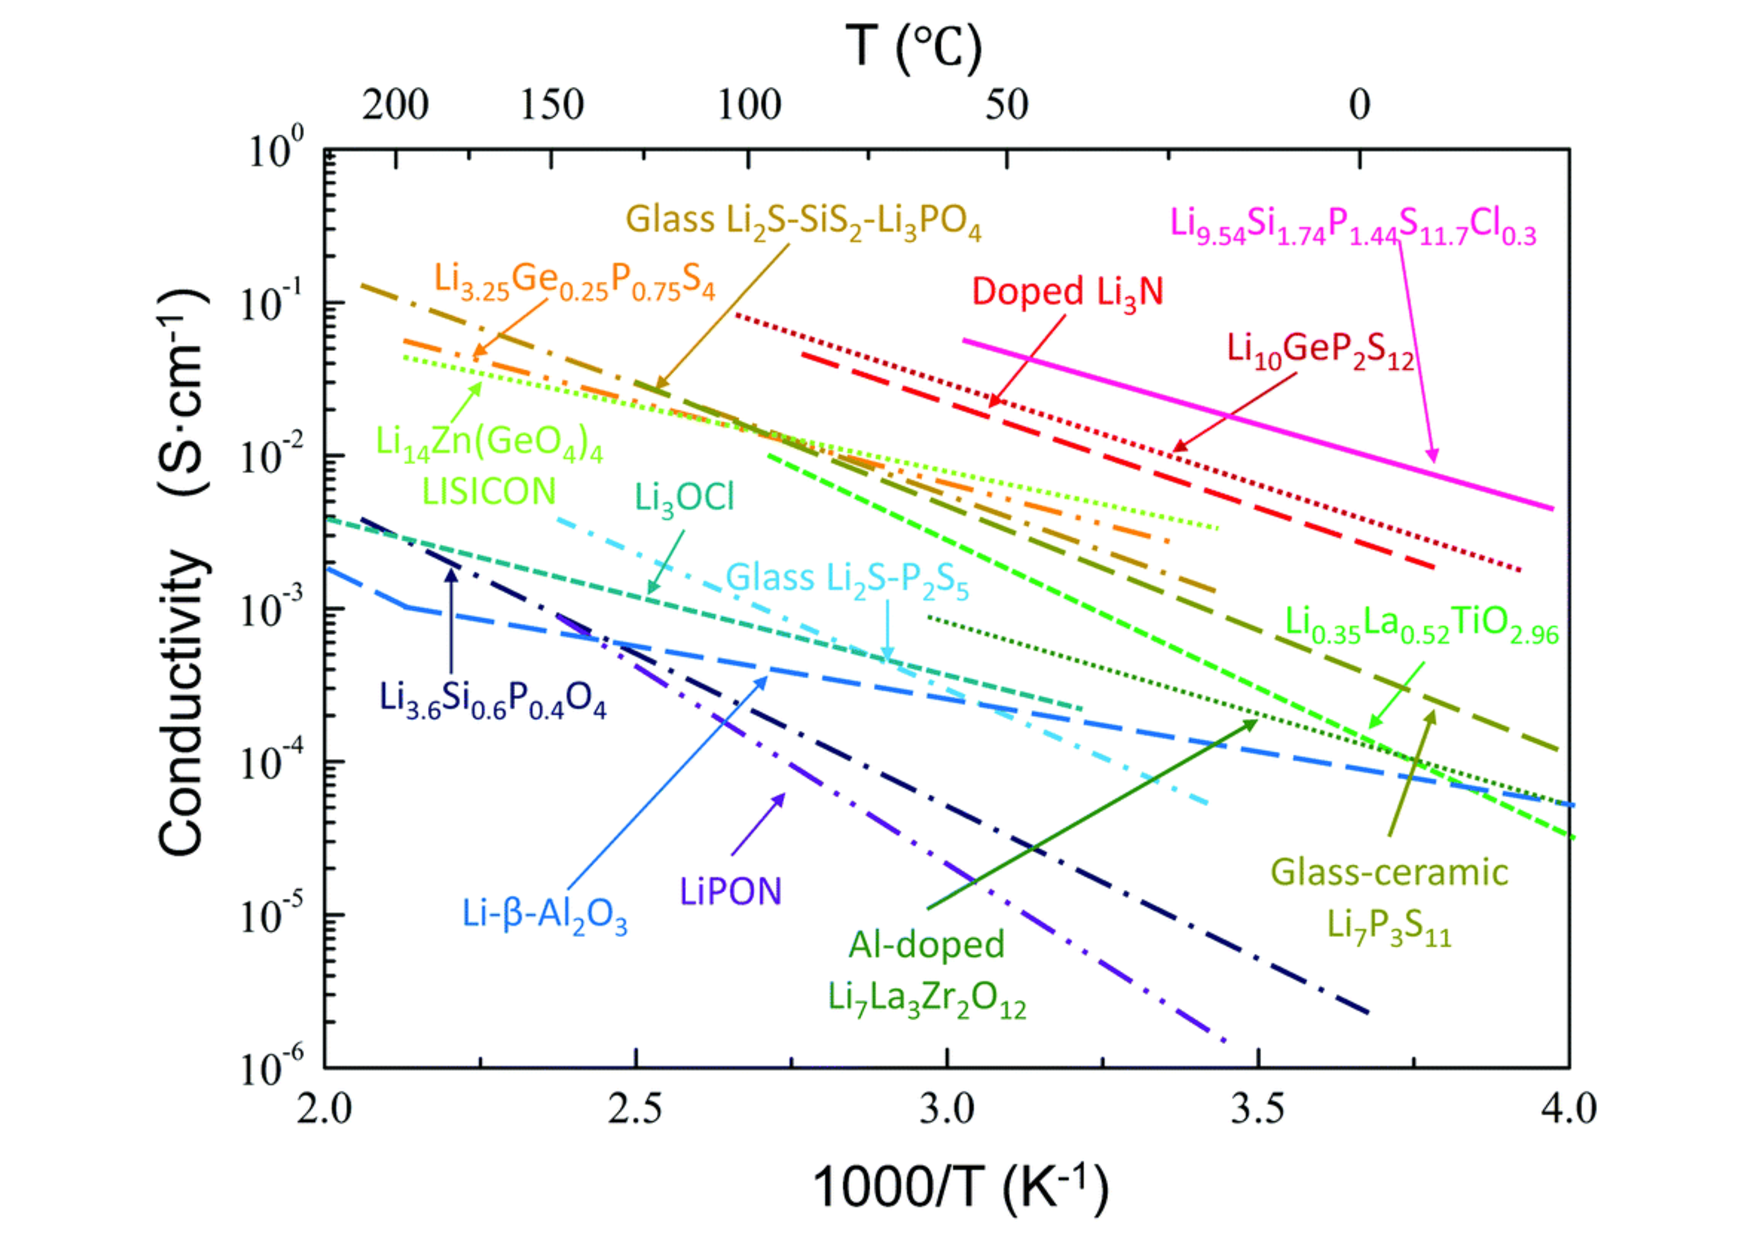
\includegraphics[scale=0.55]{figures/solid_electrolytes.pdf}
    \caption{Ion conductivity of several well-known solid lithium ion conductors, including glass and crystalline conductors. Reproduced from Ref.~\citenum{Zhang2018se_review} - Published by The Royal Society of Chemistry.}
    \label{fig:conductivity}
\end{figure}

In this section, we review atomistic modelling investigations into the structure-property relationships in selected solid-state electrolytes; Li$_{10}$GeP$_2$S$_{12}$ (LGPS), lithium argyrodites, and Li$_7$La$_3$Zr$_2$O$_{12}$ (LLZO) which belong to the inorganic solid ceramic electrolyte type and Li$_{2}$O:B$_{2}$O$_{3}$ materials which belong to the oxide based solid composite type. A particular focus is given on the ion transport mechanism in those materials, which is important for reaching high conductivities, a key property of battery materials. Finally, we take a more detailed look at the interface of solid electrolytes with the electrodes, and discuss the challenges and outlook for future atomistic modelling investigations.

\subsubsection{Sulfides (Arihant/Lucy)}
There are a substantial number of computational studies of sulfides which largely related to a recent increase in newly discovered crystalline sulfide superionic conductors. Sulfides also tend to have comparatively lower intrinsic electrochemical and chemical stability, which has stimulated interest in understanding the interfacial interactions within batteries. \cite{Xiao2020interfacerev} The sulfide group encompasses a range of sulfide based solid electrolytes, including, glass ceramics \cite{minami2006recent}, argyrodites \cite{bai2020research}, and thio-LISICONs \cite{minafra2020two}. Some of the most promising SEs to emerge in recent years include the Li$_{10}$GeP$_2$S$_{12}$ (LGPS) \cite{Bhandari2016,Kamaya2011,Mo2012} and the Li-argyrodite (Li$_6$PS$_{5}X$, $X$=Cl,Br,I) \cite{kraft2018,deiseroth_li6ps5x_2008,deklerk2016,kraft2017,minafra2018,adeli2019} families of superionic conductors.

\textbf{LGPS}
A study by \citeauthor{Kamaya2011} reports Li$_{10}$GeP$_2$S$_{12}$ (LGPS) can reach high room temperature ionic conductivities of 12 mS cm$^{-1}$, comparative to commercial liquid electrolytes.\cite{Kamaya2011} The authors also determined diffusion in LGPS is anisotropic, where $c$ directional motion is predominant over the $ab$ plane, with an overall energy barrier for Li diffusion being 0.24 eV, with later reports measuring 0.22 eV.\cite{Kuhn2013b} Using \textit{ab initio} MD \citeauthor{Mo2012} later determined the average direction energy barriers of 0.17 eV along the $c$ channel and 0.28 eV in cross channel ($ab$ plane), \cite{Mo2012} with \citeauthor{Xu2012one} showing the Li migration mechanism is through cooperative motion instead of the initially determined single-hop mechanism.\cite{Xu2012one} More recently, \citeauthor{Adams2012} predicted the presence of additional Li sites using MD, which would allow diffusion along the $ab$ plane.\cite{Adams2012} These sites could change not only the Li occupancies in the $c$ channel, but also provide a diffusion mechanism involving $ab$ plane, opening up the possibility of cross-channel diffusion. The presence of these additional sites were later confirmed experimentally using single crystal XRD.\cite{Kuhn2013a}

More recently, \citeauthor{Bhandari2016} also investigated the lithium diffusion dimensionality in LGPS by performing a \textit{First Principles} DFT study of the lithium diffusion energy barrier using the nudged elastic band (NEB) method.\cite{Bhandari2016} In this study the authors took into account the fractional occupancies leading to variable $c$ channel Li populations, variable chemical environments surrounding Li, and all possible migration mechanisms. The authors found that lithium diffusion is neither purely $c$ directional nor purely along the $ab$ plane, but there exists a correlated mechanism of motion along $c-ab$ which critically controls the degree of anisotropy of Li diffusion in LGPS. The energy barriers for different mechanisms of Li-diffusion, shown in Figure~\ref{fig:lgps}, suggest correlated hopping has the lowest energy barrier. %This correlated mechanism of Li-diffusion could not be deciphered from the experimental data or MD data alone, as these methods can only isolate diffusivities along particular directions. 
\citeauthor{Bhandari2016} further performed a statistical average of all diffusion energy barriers, taking into account the formation energy of various Li configurations and predicted an overall energy barrier of 239 meV, which is in close agreement with experiments.\cite{Kamaya2011} Thus, the \textit{First Principles} approach not only explained the overall diffusivities and energy barriers, but also gave insight into the underlying mechanism behind the fast Li diffusion in LGPS and resolved the discrepancy about the anisotropy of Li diffusion in this compound.

\begin{figure}
    \centering
    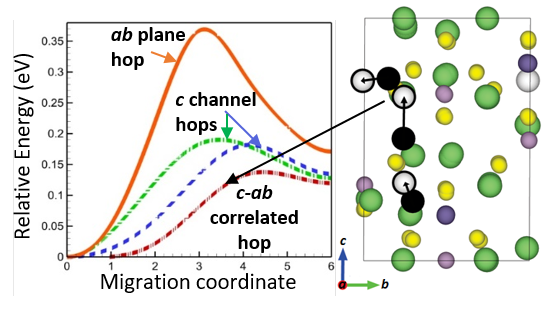
\includegraphics[scale=1.2]{figures/lgps.png}
    \caption{Energy barrier for Li-ion diffusion in LGPS solid electrolyte calculated using NEB method. Reprinted with permission from Ref.~\citenum{Bhandari2016}. Copyright 2016 American Chemical Society.}
    \label{fig:lgps}
\end{figure}

\textbf{Lithium argyodites}, Li$_6$PS$_{5}X$ ($X$= Cl,Br,I) can reportedly reach ionic conductivities of up to $10^{-2}$ Scm$^{-1}$. \cite{deiseroth_li6ps5x_2008} While Li$_6$PS$_{5}$Cl and Li$_6$PS$_{5}$Br exhibit high ionic conductivities of $10^{-3}$ Scm$^{-1}$ at room temperature, Li$_6$PS$_{5}$I has considerably lower conductivitives of $10^{-6}$ Scm$^{-1}$.The three orders of magnitude difference is surprising as the identical crystal structures suggest the same Li diffusion pathways exist in all systems. Another intriguing aspect is that the conductivity trend runs counter to other families of SEs, such as LGPS, where larger, more polarisable and less electronegative anions are linked with increased ionic conductivites. \cite{bachman2016inorganic}

Understanding which properties and mechanisms influence the conductivity is essential to obtaining higher ionic conductivities and improving battery performance. Material stoichiometry, anion/cation disorder, and doping, have all been shown to influence conductivities. The effect of these can be difficult to deconvolve in many materials as they are intrinsically coupled in experimental systems. This is where computational analysis can provide vital insight, allowing deconvolution of coupled properties and the roles they play in the diffusion process.

A particularly interesting aspect of the Li-argyrodites is the diffusion topology, which comprises of interconnected Li$_6$S cages, with anions arranged at 4a, 4c, and 16e Wyckoff positions and Li arranged over type 1, 2, 4, and 5 tetrahedra.\cite{kuhs1979} Lithium mainly occupies type 5 tetrahedral sites in $x$(Li)=6 argyrodites, with occupation of non-type 5 sites only recently observed experimentally. \cite{ohno2019further,gautamengineering} Computational studies however have previously predicted occupation of non-type 5 sites, showing lithium distributed over tetrahedral types 5, 2, and 4. \cite{deiseroth_li6ps5x_2008, Minafra2020, morgan2020mechanistic}

Li hopping within these cages, while effectively barrier-less, does not contribute to long-range diffusion. In fact, a combination of inter-cage and intra-cage hopping is needed, with occupation of non-type 5 sites and transitions between all adjacent site types to achieve long-range diffusion. This is shown schematically in Figure~\ref{fig:diffusion_pathways} showing the connectivity between the Li tetrahedral sites. AIMD simulations have shown that cation and anion substitution \cite{ohno2019further,deklerk2016}, anion site disorder \cite{gautamengineering,morgan2020mechanistic}, and lithium concentration \cite{Deng2017, yu_superionic_2020, Feng_2020}, all influence the ionic conductivity.

\begin{figure}
    \centering
    
\includegraphics[scale=0.65]{figures/diffusion_pathways.pdf}
    \caption{(a) Possible Li diffusion pathways in Li-argyrodites involving types 2, 4, and 5 tetrahedra for long range diffusion. Reprinted with permission from Ref.~\citenum{morgan2020mechanistic}. Copyright 2020 American Chemical Society.}
    \label{fig:diffusion_pathways}
\end{figure}

The influence of anion substituent concentration on conductivity is currently uncertain, with research by \citeauthor{deklerk2016} determining excess Cl in Li$_5$PS$_4$Cl$_2$ resulting in similar conductivities to Li$_6$PS$_5$Cl \cite{deklerk2016}, in contrast to research by \citeauthor{yu2019tailoring} and \citeauthor{Feng_2020} concluding excess Cl improved Li conductivity. \citeauthor{yu2019tailoring} determined the highest conductivity was produced by Li$_{5.7}$PS$_{4.7}$Cl$_{1.3}$ (6.4 mS cm$^{-1}$), \cite{yu2019tailoring,yu_superionic_2020} while \citeauthor{Feng_2020} determined this to be Li$_{5.3}$PS$_{4.3}$Cl$_{1.7}$ (17 mS cm$^{-1}$). \cite{Feng_2020} \citeauthor{Feng_2020}, however, presented alternative, or coupled, reasoning for this increased conductivity. Drawing from previous studies \cite{adeli2019,zhou_solvent-engineered_2019} they propose the increased Cl content amplified the anion disorder in the system, which is the underpinning cause of the higher conductivities.

\subsubsection{Oxides (Julian/Rana)}
\label{sec:se_oxides}
\textbf{LLZO} Cubic Li$_7$La$_3$Zr$_2$O$_{12}$ (c-LLZO) has a high Li-ion conductivity of 10$^{-4}$ Scm$^{-1}$\cite{Murugan2007}, a high shear modulus of 59 GPa\cite{Ni2012}, and the largest thermodynamic stability window with reference to lithium metal\cite{Zhu2016, Zhu2015, Binninger2020} of current solid electrolyte materials (c.f. section~\ref{sec:interface_stability}). However, at low temperatures ($<150^\circ$C) c-LLZO is not stable and transitions to the less conductive tetragonal LLZO (t-LLZO) phase.\cite{Geiger2011} Attempts have been made to retain the more desirable c-LLZO by Al doping on lithium sites, with some success.\cite{Geiger2011, Rangasamy2012}

Lithium dendrite growth has been shown to be a challenge in solid-electrolytes. For LLZO, dendrite growth has caused short circuits in the cells after relatively short periods\cite{Ren2015,Sudo2014}. \citeauthor{Cheng2017} observed this growth directly and found the process occurs mostly through grain boundaries.\cite{Cheng2017} Recently, \citeauthor{Kim2020} confirmed these observations and investigated the use of an interlayer buffer to restrict Li propagation through grain boundaries.\cite{Kim2020}

There has been a wide effort to understand dendrite formation through modelling\cite{Canepa2018, Tian2018, Gao2020}. For example, \citeauthor{Tian2018} used DFT to investigate dendrite growth through analysis of c-LLZO and t-LLZO bulk and slab surface energies via the total density of states (TDOS) \cite{Tian2018}. The authors found that t-LLZO forms at the surface of bulk c-LLZO, even with Al-doping\cite{Ma2016, Rettenwander2018}, and extra states appear in the band gap for the slab structures, which do not appear in the bulk, potentially allowing electrons to be trapped on the surface of LLZO. Electrons localised primarily around Li$^+$ and La$^{3+}$ ions on the surface lead to the nucleation of lithium metal, which can result in lithium growth through grain boundaries and pores in the LLZO, eventually forming dendrites\cite{Ren2015}, as shown in Figure~\ref{fig:tian2020}. This analysis was also conducted on Li$_2$PO$_2$N (LiPON), where no electron trapping was found to occur, indicating that LiPON could be a suitable coating to prevent dendrite and t-LLZO formation (c.f. section \ref{sec:interface_stability}).

\begin{figure}[H]
    \centering
    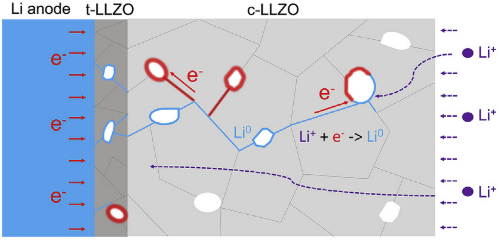
\includegraphics{figures/tian_grain_growth.png}
    \caption{Schematic showing Li metal formation (blue) along grain boundaries and pores due to electron accumulation (red) combining with Li$^+$ as they move through the electrolyte. Reprinted from Ref.~\citenum{Tian2018}, Copyright 2018, with permission from Elsevier.}
    \label{fig:tian2020}
\end{figure}

\citeauthor{Gao2020} attributed the dendrite growth mechanism to the under-coordination of Zr present on some of the stable interfaces of LLZO with Li,\cite{Gao2020} leading to inhomogenous Li depletion, which has been linked to Li metal deposition and dendrite formation. It is unclear whether the suggested cause by \citeauthor{Gao2020} is complementary evidence of \citeauthor{Tian2018}'s electron trapping theory or a separate cause of interface dendrite growth. However, the papers do differ on the choice of surface. \citeauthor{Tian2018} used Li and La rich surfaces, which were determined to be more stable by \citeauthor{Thompson2017}, who used DFT to investigate 6 different LLZO slabs for the (100) and (110) planes.\cite{Thompson2017} In contrast, \citeauthor{Gao2020} drew upon results presented in several methods\cite{Thompson2017, Canepa2018, Yu2016a} and performed DFT calculations on a wider range of surfaces, finding (100) and (001) surfaces to be the most stable. The findings of these studies agree that Li and La rich surfaces are the most stable. However, \citeauthor{Gao2020} calculated the interface formation energies of the Li-LLZO interfaces using the CALYPSO interface structure prediction method\cite{Wang2012, Gao2019}. This method determined the Zr-rich surfaces to be the most stable. Experimental observations corroborate these findings, also determining Zr to cause interfacial degradation\cite{Zhu2019}.

Experimental measurements have suggested a non-uniform distribution of current on the surfaces as a possible cause of dendrite growth.\cite{Han2019_dendrite, Aguesse2017} Non-uniform current distribution produces random, local spikes in current density for short periods of time leading to a reduction of Li at these sites.  \citeauthor{squires_2020} used DFT to model the electronic conductivity in LLZO to probe the importance of the surface current to dendrite formation.\cite{squires_2020} The authors determined that at room temperature, bulk c-LLZO was found to have negligible electron/electron-hole concentrations, indicating that bulk defects are not a significant factor in dendrite growth. However, these models did not account for other forms of defects, such as grain boundary and surface effects. 

Understanding Li-ion migration is key to improving battery conductivity. \citeauthor{Xu2012} analysed the Li-ion migration path through LLZO using DFT with the nudged elastic band (NEB) method (c.f. section \ref{sec:methods_neb}).\cite{Xu2012} Two migration paths were observed, depending on Li concentration. Low Li$_x$ (Li$_5$La$_3$Zr$_2$O$_{12}$) led to a higher energy, single hop, migration path, whereas higher Li$_x$ (Li$_7$La$_3$Zr$_2$O$_{12}$), led to a lower energy, two hop, migration path. Using potentials-based MD (c.f. section \ref{sec:molecular_dynamics}) \citeauthor{Burbano2016} further investigated the Li-ion transport mechanisms by comparing ionic conductivity in t-LLZO and c-LLZO.\cite{Burbano2016} The authors found the longer time scale of potentials-based MD allowed the observation of a large sample of diffusion events in both LLZO structural forms. Diffusion events in t-LLZO were less common and mostly involved exactly 8 Li ions, which corresponds to the cyclic movement of Li ions around the 12 octahedral and tetrahedral ring sites in t-LLZO. This cyclic mechanism results in no net long-ranged diffusion of Li and hampers the ability of t-LLZO to conduct ions. AIMD (c.f. section \ref{sec:molecular_dynamics}) investigations of the transport mechanism in LLZO have been conducted. However, the shorter time-scale led to some key disagreements about the transport mechanism in c-LLZO.\cite{Meier2014, Jalem2013, Burbano2016}

DFT calculations have determined Al doping reduces the energy barrier for Li-ions to move between octahedral and tetrahedral sites, increasing the ionic conductivity.\cite{Rettenwander2014, Rettenwander2016} More recent work by  \citeauthor{Bonilla2019}, using potentials-based MD, supports these findings, finding increased conductivity in t-LLZO due to the Al forcing Li ions into previously inaccessible tetrahedral sites.\cite{Bonilla2019} The authors also found Al doping in c-LLZO led to a slight decrease in conductivity. They attributed this to the tendency for Al to ``trap'' Li ions close to the dopant.

\textbf{Oxide Nanocomposites} Due to attractive mechanical, electrical, optical, and magnetic properties nanocomposite oxide materials represent a new generation of advanced materials. \cite{uvarov2011,Heitjans_2003} They often show enhanced conductivity compared to the single-phase ceramic oxides which makes them suitable candidates as electrolytes for future solid state batteries. For example, Li$_2$O:B$_2$O$_3$ \cite{Heitjans_2003,Indris2000,Indris2002} and Li$_2$O:Al$_2$O$_3$ nanocomposites \cite{B300908D} have higher ionic conductivities than nanocrystalline Li$_2$O, although B$_2$O$_3$ and Al$_2$O$_3$ are insulators. The ionic conductivity shows a maximum at about 50 \% of B$_2$O$_3$/Al$_2$O$_3$ content. This surprising behaviour was attributed to the increased fraction of structurally disordered interfacial regions and the enhanced surface area of the nanosized particles \cite{Heitjans_2003}. The oxide nanocomposites contain three types of interfaces, as presented in Fig.~\ref{fig:LBO} (a): interfaces between the ionic conductor grains (green lines), between the insulator grains (black lines), and between the ionic conductor and the insulator grains (red lines). The latter can lead to surprising effects in the conductivity of composite materials. In this case, the highly conducting interface region can act as a bridge between two Li$_2$O grains not in direct contact with each other, opening up additional paths for Li ions. The conductivity enhancement in the interfacial regions may have different origins, e.g. the formation of space charge layers, an enhanced concentration of dislocations, or defects or the formation of new phases.

\begin{figure}
    \centering
    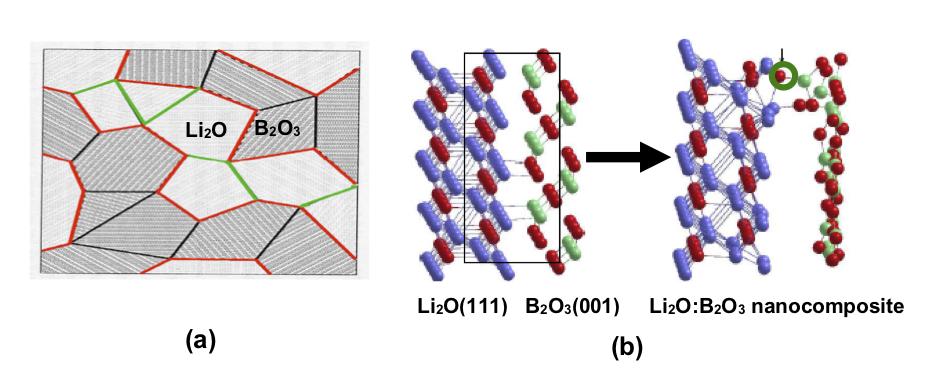
\includegraphics[scale=1]{figures/Islam-Fig-Li2O-B2O3.png}
    \caption{(a) Schematic diagram of Li$_2$O and B$_2$O$_3$ interface (b) Atomistic model of Li$_2$O:B$_2$O$_3$ nanocomposite. Reproduced with permission from Ref.~\citenum{Rana-JPCM-2012} Copyright IOP Publishing. All rights reserved.}
    \label{fig:LBO}
\end{figure}

\citeauthor{Rana-PRL-2007} studied the interface of Li$_2$O:B$_2$O$_3$ nanocomposite by modelling a combination of two favorable surfaces of Li$_2$O and B$_2$O$_3$ using HF/DFT Hybrid approach. \cite{Rana-PRL-2007,Rana-JPCM-2012} After full structural optimisation, it was observed that Li--O bonds are weakened and simultaneously B--O bonds are formed at the boundary between the two surfaces, Fig. \ref{fig:LBO} (b). An oxygen atom from the Li$_2$O surface (marked by a green circle) is pulled from the surface layer towards a neighboring boron atom of the B$_2$O$_3$ surface. This preference of oxygen bonding with B (or Al in Li$_2$O:Al$_2$O$_3$) plays a key role in generating low-coordinated Li. As a consequence of this dislocation, the coordination of a Li atom in the second layer is reduced from four to three. 

The defect properties were investigated in the interface region. It was observed that the removal of surface oxygen from Li$_2$O is responsible for the increased vacancy defect concentration in Li$_2$O:B$_2$O$_3$ (or Li$_2$O:Al$_2$O$_3$) nanocomposite materials. Therefore the nanocomposites of ionic compounds (containing weakly bound and therefore mobile cations) with highly covalent compounds (with strong metal- or nonmetal-oxygen bonds) are in general promising candidates for high ionic conductivity. The model calculations showed that the most likely mechanism for Li$^+$ migration was in a zigzag pathway rather than in a straight line along a direction parallel to the interface plane. 

The average calculated activation energy for Li$^+$ migration in the Li$_2$O:B$_2$O$_3$ interface (0.28 eV) \cite{Rana-PRL-2007,Rana-JPCM-2012} is similar to the experimental values of bulk Li$_2$O (0.31 eV) \cite{Heitjans_2003}, Li$_2$O:B$_2$O$_3$ ($0.34 \pm 0.04$ eV) \cite {Indris2002} and Li$_2$O:Al$_2$O$_3$ ($0.30 \pm 0.02$ eV) \cite{B300908D} nanocomposites. According to the defect formation energies, the interface region of Li$_2$O:B$_2$O$_3$ nanocomposites contains higher concentrations of both Li vacancies and Frenkel defects than bulk Li$_2$O and the Li$_2$O surfaces. \cite{Rana-PRL-2007,Rana-JPCM-2012} Therefore the experimentally observed enhanced Li mobility in the Li$_2$O:B$_2$O$_3$ interface region is thermodynamically and not kinetically controlled. Models as proposed in that study allowed a direct simulation of the defect formation and ion mobility at atomic scale without any experimental input. They provided a deep insight into the local bonding situation at the interface of oxide nanocomposites which was difficult to obtain from experiments.

\subsubsection{Interface stability (Julian)}
\label{sec:interface_stability}
Experimental investigations of solid electrolyte interfaces are often challenging, making atomistic modelling a vital tool.\cite{Xu2018exp} The interface stability properties of solid electrolyte materials in contact with an electrode are best described by its electrochemical stability window. The electrochemical stability window is defined by \citeauthor{Zhu2016} as the range of voltages under which the interface configuration, which is a mixture of electrode (Li) and the solid electrolyte, does not undergo a decomposition reaction.\cite{Zhu2016}

It has been widely reported in both experiment\cite{Liu2013, Han2015} and theory\cite{Mo2012} that certain solid electrolytes have an electrochemical stability window with reference to a Li anode between 0--5 V.\cite{Kamaya2011, Thangadurai2005, Liu2013} \citeauthor{Mo2012} reported a 3.6 eV band gap from a DFT calculation (c.f. section~\ref{sec:dft}) for LGPS,\cite{Mo2012} attributing the higher solid electrolyte stability observed to the passivisation phenomenon forming an interphase layer at the interface of the anode-electrolyte.\cite{Kobayashi2008} More recent work by \citeauthor{Zhu2015} has questioned this high stability window, using DFT to demonstrate that the stability windows, particularly of sulfides, are far smaller than originally thought (Figure~\ref{fig:se_stab}).\cite{Zhu2015} 

A smaller thermodynamic window increases the importance of the interphase layer formation. \citeauthor{Zhu2015} determined that a range of solid electrolytes are unstable with respect to Li metal at low and high voltages, with the exception of LLZO, which appears to be kinetically stabilised at low voltages due to an unfavourable reduction energy of -0.02 eV per atom. Any potential outside of the thermodynamic stability window results in decomposition into lithium binary compounds unless otherwise kinetically stabilised. This is problematic for germanium and titanium containing compounds as they form electronically conductive alloys upon decomposition.\cite{Zhu2015} This renders the proposed passivation process impossible\cite{Mo2012, Zhu2015} as this degradation process would be sustained throughout the bulk cycling, severely limiting the efficacy of these materials as electrolytes. Such degradation can also increase interfacial resistance\cite{Takada2008, Sakuda2010}. Other solid electrolytes face different problems. As explained in sec. \ref{sec:se_oxides}, LLZO forms the far less ionically conductive tetragonal LLZO at the surface. The Li-LiPON and Li-argyordites interfaces were reported to degrade favourably, forming an ionically conductive and electronically insulating interphase consisting of Li$_2$O, Li$_2$S, Li$_3$P, Li$_3$N, and LiI.\cite{Zhu2015} 

\begin{figure}[H]
    \centering
    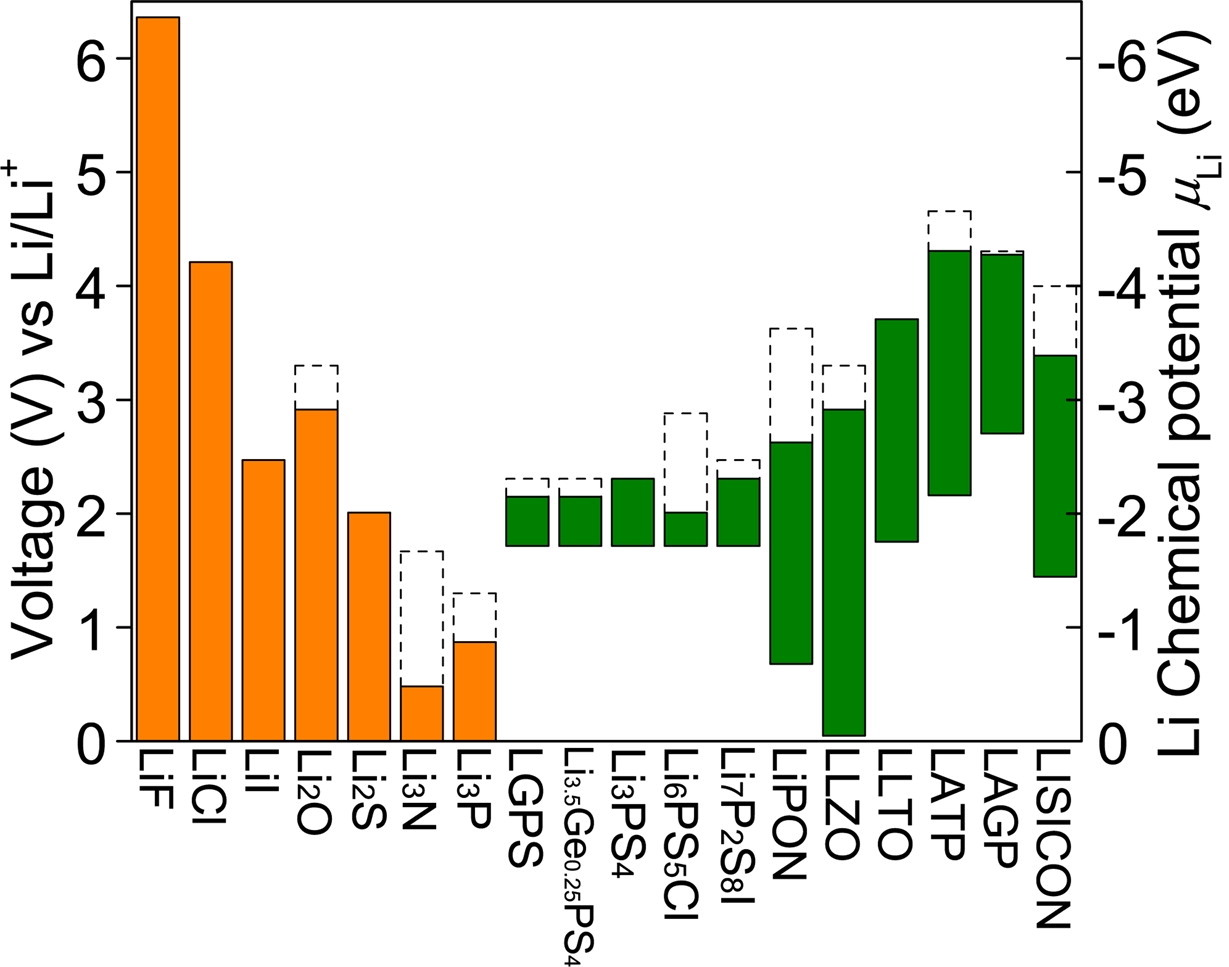
\includegraphics[scale=0.45]{figures/zhu2015_electrochemical_windows.png}
    \caption{A comparison of the voltage stability windows for a selection of solid electrolytes (green) and the binary compounds that often form upon decomposition of the solid electrolyte (orange). The dashed line represents the oxidation potential to fully delithiate the material. Reprinted with permission from Ref.~\citenum{Zhu2015}. Copyright 2015 American Chemical Society.}
    \label{fig:se_stab}
\end{figure}

Further study by \citeauthor{Zhu2016} sought to investigate the mechanism behind the degradation/instability at the surface.\cite{Zhu2016} In order to probe these mechanisms, the authors looked at several solid electrolytes (LGPS, LLZO, LiPON, NAISICON-type, LLTO) and calculated their chemical stability, electrochemical stability, and the equilibrium conditions at the interfaces. Examining the cathode-electrolyte interface, using lithium cobalt oxide (LCO) as the cathode, a similar pattern emerged: oxides were found to be far more stable than their sulfide counterparts. However, LLTO and LATP had the best electrochemical stability against LCO.

Studies looking into the interfacial resistance have been conducted,\cite{Tateyama2019, Okuno2020, Sharafi2017, Jiang2019} with the main source of resistance attributed to the electric double layer, which in liquid electrolytes consists of a capacitance and diffusion layer (c.f. section~\ref{sec:electrolytes_introduction}).\cite{Tateyama2019} %The EDL in solid electrolytes is made up of a space charge layer of point defects in ionic materials (Figure~\ref{fig:se_edl}). \cite{Swift2021} 
\citeauthor{Tateyama2019} use the CALYPSO method to find low-energy surfaces\cite{Gao2019} to probe the interface. The lithium chemical potential of these stable interfaces in the Helmholtz layer, corresponding to the negative of the Li ion vacancy formation energy, was determined. These energies correspond to lithium moving from the electrode to the electrolyte, with the vacant lithium sites becoming a potential source of interfacial resistance. \citeauthor{Okuno2020} use DFT calculations to compare the interfacial resistances of sulfide and oxide based solid electrolytes with LCO cathodes.\cite{Okuno2020} The Li vacancy formation energy at various interfaces and ion exchange across the interface were calculated. It was found that sulfide based electrolytes had a higher interfacial resistance, due to the presence of more sites with a low vacancy formation energy on the surface. The authors also found the interfacial resistance to be dependent on the orientation of the crystals at the interface. The cause of interfacial resistance can also be attributed to preparation of solid electrolyte surfaces.

% \begin{figure}
%     \centering
%     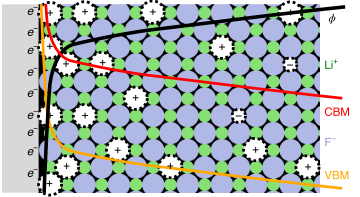
\includegraphics{figures/SE_EDL.png}
%     \caption{Formation of an electric double layer (EDL) occurs as excess electrons on the anode are balance by the increased occurrence of positive point defects in the solid electrolyte. The conduction band minimum (CBM) and valence band maximum (VBM) are shown to demonstrate the band-bending effects the increased point defect density has on the electronic structure. $\phi$ is the electrostatic potential. \cite{Swift2021} Reproduced with permission from Springer Nature: Ref~\citenum{Swift2021}, Copyright 2021.}
%     \label{fig:se_edl}
% \end{figure}

A study by \citeauthor{Lepley2015} used DFT to investigate the interface energies between the Li electrode and the compounds that make up the interphase layer of the electrolyte.\cite{Lepley2015} They defined the interface energy as:

\begin{equation}
    \gamma_{ab}(\Omega)=\frac{E_{ab}(\Omega,A,n_a,n_b)-n_aE_a-n_bE_b}{A},
\end{equation}

where $\Omega$ is the interface configuration of atoms, $E_{ab}$ is the energy of the complete system, $E_x$ is the bulk energy per for formula unit and $A$ is the surface energy. Because the interface energy is intensive, calculating larger systems will give a converging value for $\gamma_{ab}$,

\begin{equation}
    \lim_{\Omega_s \rightarrow \Omega} \left[\gamma_{ab}(\Omega_s)\right]=\gamma_{ab}(\Omega),
\end{equation}

where, $\Omega_s$ is the atomic configuration in a sample of the interface volume. Because the exact matching of lattice constants between interfaces is unlikely, a semi-coherent interface is considered, meaning lattice strain needed to be taken into accounted. Using the lowest overall lattice energy structure and explicitly accounting for the lattice strain, the most probable interfaces could be found. The Li/Li$_3$PO$_4$, Li/Li$_2$O and Li/Li$_2$S interfaces were found to be stable and the Li/Li$_3$PS$_4$ interface was found to be unstable.\cite{Lepley2015}

In response to the apparent poor stability of most solid electrolytes, many studies have attempted to simulate the effect of coating the electrolyte with an oxide layer\cite{Zhang2020directvis, Xiao2019coat, Tian2018}. As discussed in section~\ref{sec:se_oxides}, \citeauthor{Tian2018} identified LiPON as a suitable coating material for LLZO by comparing the bulk and surface density of states\cite{Tian2018}. The authors found no extra states on the surface structure, so concluded that no electron trapping would occur (the primary mechanism that they attributed to dendrite formation). Recently, \citeauthor{Sang2020} proposed an artificial interphase layer between the Li anode and the solid electrolyte composed of a Li$_{3a_b}$N$_{a}X_{b}$ compound, where $X$ is a halide.\cite{Sang2020} 
This material was investigated computationally by screening stable and metastable structures using the USPEX structure prediction software.\cite{Glass2006, Oganov2006} The dynamic stability of the stable structures was found by analysing the phonon frequency spectrum by using \textsc{Phono3py} \cite{Parlinski1997, Togo2008,togo_distributions_2015}. The temperature-dependant ionic transport properties were found using \textit{ab initio} molecular dynamics (AIMD). (c.f. section~\ref{sec:molecular_dynamics})

Phase diagrams for various atomic configurations were then constructed using a cluster expansion, implemented through the Alloy-Theoretic Automated Toolkit (ATAT)(c.f. section~\ref{sec:cluster_expansion}).\cite{Hart2008, VandeWalle2002} Through these various computational techniques, \citeauthor{Sang2020} found that Li$_6$NCl$_3$ to have the most favourable properties for use with sulfide-based solid electrolytes such as LGPS.\cite{Sang2020}

\subsubsection{Outlook and challenges (Julian/Lucy)}
\label{sec:outlook_electrolytes}
The drive for the development of commercialised all-solid-state batteries has been intense, with the electric vehicle industry being at the forefront of promoting this.\cite{Woods_2021} Although solid-state batteries can offer high gravimetric energy density (250 Wh kg$^{-1}$) and volumetric energy density (700 Wh L$^{-1}$), along with improved safety over conventional liquid electrolytes, the slow ionic diffusion can impair the fast discharge and charge performance. With solid electrolytes intended to replace both the separator and liquid electrolyte in conventional LiBs, \cite{schnell2020solid} there are still multiple challenges which need to be overcome for this to be viable. In recent years there have been breakthroughs in the discovery of new solid electrolytes, such as Li$_{9.54}$Si$_{1.74}$P$_{1.44}$S$_{11.7}$Cl$_{0.3}$, \cite{kato2016high} which exhibit ionic conductivity competitive with that of organic liquid electrolytes. The improved performance of these materials is enabled by interfacial coatings or buffer layers, and micro-structure engineering solutions at the electrode/electrolyte interfaces.  \cite{kim2021solid}

There are several critical issues related to the pairing of solid electrolytes with cathode and anode materials, which need to be addressed for long-term battery operation. Solid-state batteries are currently not capable of reliable cycling at current densities $>$ 0.6 mA cm$^{-2}$\cite{famprikis_fundamentals_2019, Albertus2018}. The current density and stability is limited by: poor electrode/electrolyte physical contact leading to particle cracking and interface delamination, formation and propagation of Li dendrites, chemical and electrochemical stability, and high interfacial resistance: \cite{famprikis_fundamentals_2019} 

\begin{itemize}
    %lattice miss-match
    \item The limited system sizes of atomistic modelling are not sufficient to capture lattice relaxation, which allows a coherent (completely matched) interface to form. This amplifies the effects of lattice strain in the model, particularly in cases where periodic boundary conditions are used. \cite{Lepley2015} The lattice strain energy can be calculated and factored into bulk scale calculations but it is not as accurate as explicitly calculating dislocation defects that naturally relieve lattice strain.\cite{Rodney2017, Clouet2020}
    %Dendrite formation
    \item Dendrite formation has been a notable problem for even the most physically robust electrolytes (c.f. section~\ref{sec:se_oxides}). Modelling of dendrite formation mechanisms has yielded some contradictory results due to incomplete models of the interface \cite{Tian2018, Gao2020, Canepa2018}. However, a more detailed understanding requires modelling of larger systems, encompassing the interface and bulk regions of both materials. The entails a high computational cost not reachable through \textit{First Principles} methods. Further development of the linear-scaling DFT approach (c.f. section~\ref{sec:lsdft}) may allow more complete multi-scale approach.
    %electric double layer
    \item The system size limitations in DFT modelling also hinder the modelling of the full electric double layer, which is also applicable to liquid electrolytes. Comparatively, in solid electrolytes the double layer is less understood. For example, \citeauthor{Tateyama2019} were only able to successfully model the initial capacitance layer at the interface (Helmholtz layer).\cite{Tateyama2019}
    %interfacial resistance
    \item Interfacial resistance presents an interesting challenge as it can be introduced through multiple mechanisms\cite{Jiang2019}: electric double layer \cite{Tateyama2019}, surface crystal orientation\cite{Okuno2020}, and production issues such as poor wettability\cite{Sharafi2017}. Strong collaboration between theorists and experimentalists will be needed in order to make informed improvements to current interfacial structures.
\end{itemize}

The interface is the primary source of dendrite formation, lattice mismatch, and interfacial resistance in solid electrolytes. The interface also presents opportunities for atomistic modelling with the growing popularity of coatings that try to address the shortcomings of popular solid electrolytes.\cite{Kim2020, Xu2018exp, Chen2020se_coat, Ito2017, Yin2020, Ji2020coating, Li2020coating, Yi2021coating, Dai2021coating, Pan2020coating, Jing2020coating, Wang2021coating, Zhao2020coating, Zhao2021coating, Liang2020coating, Zhang2020coating} For example, \citeauthor{Tian2018}'s solution to dendrite growth in LLZO by utilising a LiPON coating\cite{Tian2018} (c.f. section \ref{sec:se_oxides}). Understanding how effective coatings are at addressing the aforementioned issues is essential. \cite{Zhang2020directvis, Xiao2019coat, Tian2018} A very recent review by \citeauthor{kim2021solid} presents a detailed insight into the challenges and future prospects of solid-state Li-metal batteries, which we have touched upon here.\cite{kim2021solid}
\end{document}